\documentclass[czech,master,public,dept470,male,cpdeclaration,oneside, python]{diploma}

\usepackage{subfig}		% makra pro "podobrazky" a "podtabulky"
\usepackage{tikz}		% makra pro kresleni

\usepackage{amsmath}
\usepackage{amssymb}

\usepackage{graphicx}
\usepackage{float} 
\usepackage{pgfplots} 
\graphicspath{  }
\usepackage{listings}
\usepackage{xspace}
\usepackage{color} %red, green, blue, yellow, cyan, magenta, black, white
\definecolor{mygreen}{RGB}{28,172,0} % color values Red, Green, Blue
\definecolor{mylilas}{RGB}{170,55,241}


\usepackage{xcolor}
%\newcommand\myworries[1]{\textcolor{red}{#1}}

\CzechAbstract{Práce se zabývá modelem po částech linearní regrese. Obsahuje stručný úvod do Bayesovské statistiky, dále zavádíme model pro po částech lineární regresi. Protože se s aposteriorním rozdělením dáneho modelu nedá analyticky pracovat, používáme pro jeho aproximaci algoritmus RJMCMC. K tomu se postupně dostáváme přes klasické MCMC metody. Na závěr práce prezentujeme výsledky dosažené za pomocí algoritmu RJMCMC, jehož implementace je součásti této práce a byla provedena v programovacím jazyce Python.}

\CzechKeywords{Python, Markov Chain Monte Carlo, MCMC, Reversible Jump Markov Chain Monte Carlo, RJMCM, Metropolis Hastings, Po částech lineární regrese, lineární  regrese, Bayesovská statistika, Theano, SciPy}

\EnglishAbstract{This work is about segmented linear regression. It contains a brief introduction to Bayesian statistics, then we define a model for piecewise linear regression. Posterior distribution for the model doesn't have a closed form, so we use RJMCMC algorithm to aproximate the distribution. Before introducing RJMCMC we give an overview of classical MCMC algorithms. At the end of the thesis we show examples of how RJMCMC works. We implemented the RJMCMC algorithm as part of the thesis, for that we used the programming language Python. }

\EnglishKeywords{Python, Markov Chain Monte Carlo, MCMC, Reversible Jump Markov Chain Monte Carlo, RJMCM, Metropolis Hastings, Piecewise linear regression, Segmented regression, Bayesian statistics, Theano, Scipy}


\lstset{language=python,%
    %basicstyle=\color{red},
    breaklines=true,%
    morekeywords={matlab2tikz},
    keywordstyle=\color{blue},%
    morekeywords=[2]{1}, keywordstyle=[2]{\color{black}},
    identifierstyle=\color{black},%
    stringstyle=\color{mylilas},
    commentstyle=\color{mygreen},%
    showstringspaces=false,%without this there will be a symbol in the places where there is a space
    numbers=left,%
    numberstyle={\tiny \color{black}},% size of the numbers
    numbersep=9pt, % this defines how far the numbers are from the text
    emph=[1]{for,end,break},emphstyle=[1]\color{red}, %some words to emphasise
    %emph=[2]{word1,word2}, emphstyle=[2]{style},    
}


% Dalsi doplnujici baliky maker
\usepackage{subfig}		% makra pro "podobrazky" a "podtabulky"
\usepackage{tikz}		% makra pro kresleni


% Zadame pozadovane vstupy pro generovani titulnich stran.
\ThesisAuthor{Martin Koběrský}

\CzechThesisTitle{Po částech lineární regrese}

\EnglishThesisTitle{Piecewise linear regression}

\SubmissionDate{13. července 2018}

% Pokud nechceme nikomu dekovat makro zapoznamkujeme.
\Thanks{Rád bych poděkoval panu Kracíkovi za shovívavost a trpělivost a svojí mamince za zkontrolování gramatických chyb. Pokud i přesto nějaké chyby zůstaly, chyba je jen na mojí straně. Děkuji.}

% Zadame cestu a jmeno souboru ci nekolika souboru s digitalizovanou podobou zadani prace.
% Pokud toto makro zapoznamkujeme sazi se stranka s upozornenim.
\ThesisAssignmentImagePath{images/Assignment}
  

% Zadame soubor s digitalizovanou podobou prohlaseni autora zaverecne prace.
% Pokud toto makro zapoznamkujeme sazi se cisty text prohlaseni.
% \AuthorDeclarationImageFile{Figures/AuthorDeclaration.jpg}



\begin{document}
\MakeTitlePages
\lstlistoflistings

\section{Úvod}
Volba modelu je jedním z nejtěžších a nejdůležitějších problémů, které se vyskytují ve statistice.
. Objevuje se v novějších problémech jako je rozpoznávaní obrazu, ale také při tradičnějších statických úlohách, jako jsou pravděpodobnostní směsi a nebo regresní modely. \par
V této práci se budeme zabývat po částech lineární regresí. Tím myslíme, že k vysvětlení pozorování budeme používat spojitou po částech lineární funkci, u které je ale počet zlomů neznámý a tedy neznámý počet parametrů. Po částech lineární regrese s různým počtem zlomů pak tvoří jednotlivé modely. K řešení problému využijeme Bayesovskou statistiku. Její hlavní výhodou při řešení tohoto problému je to, že přirozeně znevýhodňuje modely s vyšší dimenzí \cite{robert2007bayesian}, které ale nevysvětlují data o mnoho líp než jednodušší modely. V rámci Informace o parametrech a modelu je v Bayesovské statistice reprezentována aposteriorním rozdělením, tj. apriorní informaci a informaci z dat. \par
Protože toto rozdělení je příliš složité na to, abychom s ním mohli pracovat analyticky, budeme se muset uchýlit k aproximaci. Pro tento účel se většinou používají algoritmy Markov Chain Monte Carlo, které ale nestačí na úkoly, kde počet neznámých je jeden z parametrů modelu.  Proto využijeme algoritmus Reversible Jump Markov Chain Monte Carlo, který zobecňuje algoritmy MCMC i pro modely s proměnnou dimenzí.
\section{Bayesovská statistika}
Ve statistice jsou nejrozšířenější dva přístupy, a to frekventistický a Bayesovký. Rozdíl mezi nimi je v tom, jak se staví k parametrům daného statistického modelu. Ve statistice frekventistické považujeme data za náhodné veličiny, ale parametry daných modelů za nějaké konkrétní, avšak neznámé hodnoty. Ve statistice Bayesovské považujeme i tyto parametry za náhodné veličiny. Rozdělení těchto náhodných veličin nazýváme apriorní \cite{robert2007bayesian}. Pomocí apriorního rozdělení můžeme do modelu zanést naši předchozí zkušenost nebo informaci, která není obsažena v samotných pozorováních. Nyní zavedeme zmíněné náhodné veličiny a jejich pravděpodobnostní hustoty:
\begin{itemize}
	\item $Y = ( Y_1, ..., Y_n)$ ... data
	\item $\Theta = (\Theta_1, ... ,\Theta_p)$ ... neznámý parametr, množinu hodnot $\Theta$ budeme značit $\boldsymbol{\Theta}$
	\item $f_{\Theta}(\theta)$ ... pravděpodobnostní hustota $\Theta$, nazýváme apriorní rozdělení parametru $\Theta$ 
	\item $f_{Y|\Theta}(y|\theta)$ ... podmíněná hustota $Y | \Theta = \theta$, nazýváme parametrický model dat
\end{itemize}\par
Na základě $f_{\Theta}(\theta)$ a $f_{Y|\Theta}(y|\theta)$ můžeme pomocí Bayesovy věty odvodit podmíněnou pravděpodobnostní hustotu parametru $\theta$ za podmínky $Y=y$
\begin{align} \label{bayes}
f_{\Theta|Y}(\theta | y) = \frac{f_{Y|\Theta}(y|\theta)f_{\Theta}(\theta)}{f(y)}.
\end{align}
Toto rozdělení nazýváme aposteriorní a shrnuje veškerou informaci o parametru $\theta$, která je nám známa, tj. apriorní informaci a informaci z dat. $f(y)$ v \eqref{bayes} je marginální hustota ze sdružené hustoty $f_{Y|\Theta}(y|\theta)f_{\Theta}(\theta)$, tudíž ji lze chápat jako normalizační konstantu, která nezávisí na $\theta$ a je možné ji získat vyintegrováním čitatele v \eqref{bayes}  přes $\theta$, tj.
\begin{align*}
f(y) = \int_{\boldsymbol{\Theta}} f(y|\theta)f(\theta) d\theta.
\end{align*}
Zjednodušeně lze \eqref{bayes} zapsat ve tvaru $f_{\Theta|Y}(\theta | y) \propto f_{Y|\Theta}(y|\theta)f_{\Theta}(\theta)$, kde $\propto$ značí rovnost až na multiplikativní konstantu. \par
V dalším textu, pokud bude význam zřejmý z kontextu,
\begin{itemize}
	\item nebudeme rozlišovat náhodné veličiny a jejich hodnoty,
	\item u hustot nebudeme uvádět indexy, je-li náhodná veličina určena argumentem, tj. např $f(\theta)$ značí $f_{\Theta}(\theta)$ apod.
	\item všechny integrály chápeme jako určité přes obor hodnot příslušné náhodné veličiny.
\end{itemize}
\subsection{Bayesovská volba modelu}\label{model_choice}
V předchozí části jsme se zabývali situací s jedním konkrétním modelem, nyní se zabývejme obecnější situací, kdy máme množinu více modelů pro stejná data. Předpokládejme tedy, že máme $K$ modelů a označme $M$ index modelu, který nabývá hodnot $\{0, ..., K\}$. Z bayesovského pohledu je $M$ dalším parametrem celkového modelu dat. Pro každý z dílčích modelů předpokládáme, že data mají pravděpodobnostní hustotu $f(y |m,  \theta_m)$, kde $\theta_m$ určuje parametry modelu $m$ a toto $\theta_m$ má dimenzi $D_m$. Jinými slovy parametr celkového modelu dat $\theta = (m, \theta_m)$. Množina parametrů modelu $f(y |m,  \theta_m)$ je tedy:
\begin{align}\nonumber
\boldsymbol{\Theta} = \bigcup_{m=1}^{K} \{m\} \times \boldsymbol{\Theta}_m,
\end{align}
 kde $\boldsymbol{\Theta}_m \subset \mathcal{R}^{D_m}$ je množina hodnot parametrů modelu m. \par
Apriorní rozdělení můžeme přirozeně faktorizovat:
\begin{align}\nonumber
f(m, \theta_m) = f(m)f(\theta_m | m)
\end{align}
Aposteriorní rozdělení je opět podmíněná hustota parametru $(m, \theta_m)$ za podmínky $Y=y$:
\begin{align}\nonumber
f(m, \theta_m | y) = 
\frac{f(y | m, \theta_m)f(\theta_m | m)f(m)}{\sum_m \int f(y | m, \theta_m)f(\theta_m | m)f(m) d\theta_m}.
\end{align}
A vyintegrováním $\theta_m$ dostáváme marginální aposteriorní rozdělení pro model s indexem m:
\begin{align}\nonumber
f(m | y) =  \frac{\int f(y | m, \theta_m)f(\theta_m | m) d\theta_m f(m)}{\sum_m \int f(y | m, \theta_m)f(\theta_m | m)f(m) d\theta_m},
\end{align}
tj. podmíněnou pravděpodobnost, že data byla generována z modelu $m$, za podmínky $Y=y$.  

\section{Model}
Teoretický postup, který jsme nastínili v předchozí kapitole, budeme nyní aplikovat na po částech lineární regresi, tj. regresní model, ve kterém je regresní funkce tvořena spojitou po částech lineární funkcí. Problém, se kterým se setkáváme je, že jedním z parametrů je počet zlomů po částech lineární regrese. Jinak řečeno, jeden z parametru modelu určuje počet zbývajících parametrů. Terminologií předchozí kapitoly jde o bayesovskou volbu modelu, kde jednotlivé modely jsou regrese s různým počtem zlomů. Jak jsme si ukázali, pro odvození aposteriorního rozdělení budeme potřebovat zavést parametrické modely dat a apriorní rozdělení. Začneme u nejjednoduššího modelu a postupně přejdeme až k tomu nejobecnějšímu.
\par \par

\subsection{Model bez zlomu}

Pro určení parametrického modelu dat, vycházíme ze standardního pravděpodobnostního modelu lineární regrese: 
\begin{align}\nonumber
	y_i = a + b x_i + \epsilon_i, i =1,...,n,
\end{align}
kde $n \in \mathbb{N}$ je počet pozorování $a$, $b \in \mathbb{R}$, jsou parametry modelu. $x_i$ je hodnota vysvětlující veličiny, kterou ale považujeme za nenáhodnou. $y_i$ představuje hodnotu vysvětlované veličiny. Náhodná veličina $\epsilon_i$ představuje náhodnou chybu s rozdělením:
\begin{align*}
	\epsilon_i \sim \mathcal{N}(0, \sigma^2),
\end{align*}
kde $\sigma^2$ je neznámé. $\mathcal{N}(\mu, \sigma^2)$ označuje Gaussovo rozdělení se střední hodnotou $\mu$ a rozptylem $\sigma^2$. Dále předpokládáme, že všechny $\epsilon_i$ jsou navzájem nezávislá.
Z tohoto určíme rozdělení pro $y_i$:
\begin{align}\label{yi}
	y_i \sim \mathcal{N}(a + bx_i, \sigma^2).
\end{align}
Je vhodné dodat, že jako vysvětlovaná veličina zde vystupuje $y_i$ a $x_i$ vystupuje jako parametr, který je ale známý, proto nepíšeme, že $y_i$ je podmíněně závislé na $x_i$. Formuli \eqref{yi} můžeme také psát jako:
\begin{align}\nonumber
	f(y_i | a, b, \sigma^2) = \mathcal{N}(y_i | a + bx_i, \sigma^2)
\end{align}
Použitím $\mathcal{N}(y_i | \mu, \sigma^2)$ zapisujeme pravděpodobnostní hustotu normálního rozdělení se střední hodnotou $\mu$ a rozptylem $\sigma^2$. V tomto případě je tedy střední hodnota $a + bx_i$. Z předpokládané nezávislosti $e_i$ vyplývá nezávislost $y_i$ (za $a,b,\sigma^2$) tj:
\begin{align}\nonumber
f(y_1, ..., y_n | a,b,\sigma^2) = \prod_{i=1}^{n} f(y_i|a,b,\sigma^2).
\end{align}
\par
Takto jsme získali parametrický model dat. Nyní potřebujeme určit apriorní rozdělení.
Pokud není důvod volit apriorní rozdělení jinak, volíme konjugované apriorní rozdělení, což znamená, že aposteriorní rozdělení bude stejného typu jako apriorní rozdělení \cite{robert2007bayesian}. Apriorní rozdělení můžeme faktorizovat takto:
\begin{align}\nonumber
	f(a, b, \sigma^2) = f(\sigma^2)f(a,b | \sigma^2).
\end{align}
Aby bylo apriorní rozdělení konjugované lze ukázat \cite{robert2007bayesian}, že $\sigma^2$ má inverzní gamma rozdělení a $a,b za \sigma^2$ má normální rozdělení:
\begin{align} \label{apriori_inv}
	\sigma^2 \sim Inv-Gamma(\alpha, \beta), 
\end{align}
\begin{align}\label{apriori_norm}
	a, b | \sigma^2 \sim \mathcal{N}((\mu_1, \mu_2), \sigma^2\Lambda_0^{-1}),
\end{align}
kde $\alpha, \beta > 0 \mu_1, \mu_2 \in \mathbb{R}$ a $\Lambda_0 \in \mathbb{R}^{2\times2}$ symetrická pozitivně definitní jsou parametry apriorních rozdělení. Lze ukázat, že pro aposteriorní rozdělení platí $\sigma^2$ za podmínky dat má inverzní gamma rozdělení a $a,b$ za podmínky dat mají normální rozdělení, tj. $f(a,b,\sigma^2)$ splňující \eqref{apriori_inv}, \eqref{apriori_norm} je konjugované apriorní rozdělení. \par


\subsection{Model s více zlomy}
Nyní se tedy dostáváme k tomu, jak vypadá model s více zlomy. Nyní učiňme dohodu, že $m.$ modelem budeme vždy myslet model s regresní funkcí tvořenou spojitou po částech lineární funkci s $(m-1)$ zlomy. V modelu beze zlomů jsme jako parametry použili parametry $a$, $b$ z rovnice přímky a rozptyl náhodné složky $\sigma^2$. Pro více zlomů se nám jeví výhodnější model parametrizovat pomocí rozptylu $\sigma^2$, ale místo parametrů $a$, $b$ jednotlivých přímek použijeme několik bodů, které budou určovat souřadnice zlomů spojité po částech lineární funkce.  Počet bodů bude záviset na počtu zlomů, takže pokud budeme mít 1 zlom, použijeme body 3, pokud 2 zlomy, použijeme body 4 atd. Tedy parametr $\theta_m$ vypadá následovně:
\begin{align}\nonumber
\theta_m = (\sigma^2, s_{m_1}, h_{m_1}, s_{m_2}, h_{m_2}, ..., s_{m_{m+1}} h_{m_{m+1}}),
\end{align}
kde $\sigma^2$ je rozptyl náhodné složky $\epsilon_i$ a pro všechna $i$ body $s_i$ určují x-ové souřadnice bodů určujících přímku a $h_i$ určují y-ové souřadnice. $m$ je index modelu a zároveň počet zlomů. Body $(s_1, h_1)$ a $(s_{m+1}, h_{m+1})$ určují první, respektive poslední bod definující funkce. Bude-li z kontextu zřejmé, že pracujeme s modelem $m$ , budeme psát \begin{align}\nonumber
\theta_m = (\sigma^2, s_1, h_1, s_2, h_2, ..., s_{m+1} h_{m+1}),
\end{align}.
\begin{figure}
	[H]\centering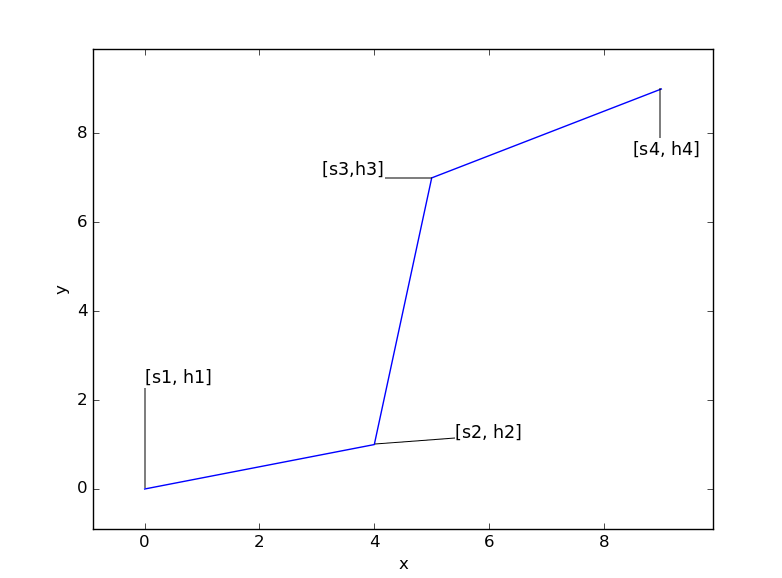
\includegraphics[width=0.8\textwidth]{images/model2.png}\caption{Znázornění parametru $\theta_2$	.}
\end{figure}
\par
Pro tento model už neexistuje konjugované apriorní rozdělení, protože parametrický model dat netvoří exponencialní rodinu \cite{robert2007bayesian}, což má za následek to že, aposteriorní rozdělení už nebude mít uzavřenou formu a my nebudeme schopni analyticky spočítat parametry nového modelu. Z toho důvodu budeme muset numericky aproximovat aposteriorní rozdělení metodami. K tomuto využijeme Markov Chain Monte Carlo\cite{robert2004monte}. Nyní popišme to, jak náš model bude vypadat. \par
Rozdíl v parametrickém modelu se zlomy oproti modelu beze zlomu je, že zde je přímka rozdělena na obecně $m$ částí, takže je třeba vzít v potaz to, kde leží bod pro který počítáme pravděpodobnost:
\begin{align}\label{parameticky_model}
f(y | m, \theta_m) = \sum_{i=0}^{m} I(s_j < X_i < s_{j+1}) 
\mathcal{N}(y - [(x - s_j)\frac{h_{j+1} - h_j}{s_{j+1} - s_j} + h_j], \sigma^2),
\end{align} \par
kde $I$ je jedna, pokud je podmínka uvnitř splněna jinak 0. Nyní zvolme apriorní rozdělení. Začneme u x-ových souřadnic $s_1, ..., s_{m+1}$ (pro m-tý model). Od těch budeme chtít hlavně to ať $s_1, ..., s_{m+1}$ tvoří rostoucí posloupnost. Když zmíněné body netvoří rostoucí posloupnost bude apriorní rozdělení nulové a v opačném případě nemáme-li další apriorní informaci, bude konstantní, tj.:
\begin{align}\nonumber
f(s_1, ..., s_{m+1}) \propto
	\begin{cases}
		1, pokud\ x_{min} \leq s_1 < s_2 < ... < s_{m+1} \leq x_{max}, \\
		0, jindy.		
	\end{cases}
\end{align}
Kde $x_{min} = min\{x_1, ..., x_n\}$ a $x_{max} = max\{x_1, ..., x_n\}$. \par
Předpokládejme, že o $h_1, ..., h_{m+1}$ nemáme žádnou apriorní informaci. Pak
\begin{align}\nonumber
f(h_1,..., h_{m+1}) \propto \prod_{i=1}^{m+1} I(y_{min} \leq y_i \leq y_{max}),
\end{align}
kde opět $y_{min} = min\{y_1, ..., y_n\}$ a $y_{max} = max\{y_1, ..., y_n\}$. \par
Pro rozptyl použijeme useknuté normální rozdělení s tím, že rozptyly menší nebo rovné nule mají nulovou pravděpodobnost:
\begin{align}\nonumber
f(\sigma^2) \propto 
\begin{cases}
\mathcal{N}(\sigma^2 | 0, q), pokud\  \sigma^2 > 0, \\
0, jindy
\end{cases}.
\end{align}
Hodnotu parametru $q$ určíme v závislosti na konkrétním příkladu.
Celé apriorní rozdělení je tedy jen pro úplnost:
\begin{align}\label{apriorni}
f(\theta_m) = f(s_1, ..., s_{m+1})f(h_1,..., h_{m+1})f(\sigma^2),
\end{align}
tj. předpokládáme nezávislost $h,s,\sigma^2$, kde $s=(s_1, ..., s_{m+1})$, $h=(h_1,..., h_{m+1})$. \par

Nyní máme parametrický model a apriorní rozdělení. Za předpokladu nezávislosti $\epsilon_i$ pak pro aposteriorní rozdělení platí:
\begin{align}\nonumber
f(\theta_m | y) \propto \prod_{i=0}^{n} f(y_i | \theta_m) f(\theta_m).
\end{align}
\subsection{Model s více zlomy a různým počtem dimenzí}
V předešlé sekci jsme popsali parametrický model a apriorní rozdělení pro pevný počet zlomů. Teď bychom chtěli najít aposteriorní rozdělení takového modelu, kde i počet zlomů je součástí parametru. Ekvivalentně je možné říct, že řešíme Bayesovskou volbu modelu, kde jednotlivé modely jsou regrese s různým počtem zlomů. Parametr $\theta = (m, \theta_m)$, kde $\theta_m \in \boldsymbol{\Theta_m}$, bude v takovém modelu vypadat následovně 
\begin{align}\nonumber
\boldsymbol{\Theta} = \bigcup_{m=1}^K\{m\} \times \boldsymbol{\Theta_m}.
\end{align}
 Nyní si zvolíme apriorní rozdělení:
\begin{align}\nonumber
f(m, \theta_m) = f(\theta_m | m)f(m).
\end{align}
Pro $m$ volíme takové rozdělení, které zvýhodňuje jednodušší modely oproti složitějším v našem případě můžeme například volit geometrické rozdělení s vhodným parametrem $e \in [0,1]$:
\begin{align}\nonumber
m \sim G(e),
\end{align}
případně můžeme volit rovnoměrné rozdělení. \par
A podmíněné rozdělení $f(\theta_m|m)$ volíme ve tvaru \eqref{apriorni}.
Parametrický model $f(y | m, \theta_m)$ pro $M=m$  volíme ve tvaru \eqref{parameticky_model}.
Pro aposteriorní rozdělení opět platí:
\begin{align}\label{supermodel}
	f(m, \theta_m | y) = f(y | m, \theta_m)f(m, \theta_m).
\end{align}
\section{MCMC}
Aposteriorní distribuce mají často takový tvar, že je jakýkoli analytický výpočet nemožný. V takový moment se buď musíme spokojit s jednodušším modelem, jehož aposteriorní distribuce umožňuje analytický výpočet a nebo se musíme uchýlit k numerickým aproximacím dané distribuce. Toto nám umožňují algoritmy Monte Carlo (MC), které dané distribuce aproximují pomocí množiny vzorků. Samotné algoritmy Markov Chain Monte Carlo (MCMC) tvoří podmnožinu algoritmů MC. Z vzorků získaných MC algoritmem můžeme například aproximovat střední hodnotu náhodné veličiny (tj. výpočet integrálu), získat přibližný intervalový odhad parametru apod. viz \cite{andrieu2003introduction}. \par
V této kapitole si nejprve ukážeme jak funguje MC integrace a poté přejdeme k Markovským řetězcům, které jsou základem MCMC algoritmů. Nakonec popíšeme nejrozšířenější MCMC algoritmus a to Metropolisův-Hastingsův algoritmus\cite{robert2004monte}.
\subsection{Monte Carlo Integrace}
Již jsme naznačili,že  myšlenkou MC simulací je aproximace distribuce náhodné veličiny $X$ s hustotou $f(x)$, definované na prostoru $\mathbb{X}$, množinou nezávislých vzorků $\{x^{(i)}\}_{i=1}^{N}$. Je tedy možné aproximovat integrály $I(h)$ posloupností výběrových průměrů $I_N(h)$, která konverguje následujícím způsobem:
\begin{align}
	I_N(h) = \frac{1}{N}\sum_{i=1}^N h(x^{(i)}) \xrightarrow{s.j.} I(h) = \int_{\mathbb{X}} h(x)f(x)dx.
\end{align}
Tedy, odhad $I_N(h)$ je nestranný odhad a podle zákona velkých čísel bude konvergovat skoro jistě k $I(h)$, tedy ... . Pokud rozptyl $h(x)$ splňuje $\sigma^2_h = E_{f(x)}(h^2(x) - (I(h))^2) < \infty$, pak je $var(I_N(h)) = \frac{\sigma^2_h}{H}$ a podle centrální limitní věty bude platit:
\begin{align}
	\sqrt{N}(I_N(h) - I(h)) \Rightarrow \mathcal{N}(0, \sigma^2_f),
\end{align}
kde $\Rightarrow$ značí konvergenci v distribuci.
\par

Chceme-li počítat integrál, kde nejde primárně o výpočet střední hodnoty, je možné jej jako výpočet střední hodnoty vyjádřit. Proto je potřeba zvolit distribuci $f(x)$, z které budeme vygenerovat vzorky. Pro výpočty integrálů s omezeným integračním oborem se jeví výhodné použít uniformní distribuci. Toto nemusí být především ve vyšších dimenzích vhodné, protože vedou k vysokému rozptylu odhadu a tedy k nutnosti použít vysoký počet vzorků. Další možnosti řešení jsou použití metod Rejection sampling, Importance sampling \cite{andrieu2003introduction} nebo v případě kdy nejsme schopni nalézt vhodnou distribuci pro generování vzorků lze použít jeden z MCMC algoritmů. \par
\subsection{Markovský řetězec}
Markovův řetězec je posloupnost náhodných veličin se specifickou strukturou podmíněných nezávislostí, k popisu podmíněných pravděpodobností se používá tzv přechodové jádro. \par
V celé této části budeme uvažovat pravděpodobnostní prostor $(\mathcal{X}, \mathcal{B}(\mathcal{X}), P)$, kde $\mathcal{X} = \mathbb{R}^n$, $\mathcal{B}(\mathcal{X})$ je borelovská $\sigma$-algebra v a $\mathcal{X}$ $P$ je pravděpodobnostní míra.
\begin{definition}
	Přechodové jádro je funkce $K: \mathcal{X} \times \mathcal{B}(\mathcal{X}) \rightarrow [0, 1]$ taková, že 
	\begin{itemize}
	\item $\forall x \in \mathcal{X}$, $K(x, \cdot)$ je pravděpodobnostní míra,
	\item $\forall A \in \mathcal{B}(\mathcal{X})$, $K(\cdot, A)$ je měřitelná.
	\end{itemize}
\end{definition}


Přechodové jádro využijeme k definici Markovova řetězce.

\begin{definition}
	Mějme přechodové jádro K, posloupnost $X_1, X_2 ...$ náhodných veličin je Markovský řetězec s přechodovým jádrem $K$, pokud pro každé $t \in \mathbb{N}$ podmíněna distribuce $X_{t+1}$ za $X_t = x_{t}, X_{t-1}=x_{t-1}, ..., X_1 = x_1$ je stejná jako distribuce $X_{t+1}$ za $X_t = x_t$, tedy:
	\begin{equation*}
		P(X_{t+1} \in A| X_t = x_{t}, X_{t-1}=x_{t-1}, ..., X_1 = x_1) = P(X_{t+1} \in A| X_t = x_t) \\.
	\end{equation*}
	a dále platí $ P(X_{t+1} \in A| X_t = x_t) = \int_A K(x_t, dx)$. \\

\end{definition} \par
Poznámka: Pro takto definovaný Markovský řetězec platí pro každé $A \in \mathcal{B}(\mathcal{X}), x \in \mathbb{X}$ a $t \in \mathbb{N}$ platí: $P(x_{t+1} \in A | X_t = x)$. Řetězec s touto vlastností se označuje jako homogenní. \par
Je-li $\mathcal{X}$ nejvýše spočetná množina, přechodové jádro lze charakterizovat přechodovou maticí K s prvky
\begin{equation*}
K_{xy} = P(X_t = y| X_{t-1} = x), x, y \in (\mathcal{X}).
\end{equation*}

Ve spojitém případě lze jádro vyjádřit jako podmíněnou hustotu $\mathcal{K}(x, x^{,}):\mathbb{R}^n \times \mathbb{R}^n \rightarrow \mathbb{R}$ přechodu $K(x, \cdot)$, tedy $P(X \in A| x) = K(x, A) = \int_A \mathcal{K}(x, x^{,}) dx^{,}$. 


Pro využití v MCMC jsou důležité dvě vlastnosti Markovovských řetězců a to neredukovatelnost a aperiodicita. Neredukovatelnost zjednodušeně říká, že Markovovský řetězec se někdy dostane do každého možného stavu nezávisle na tom v jakém stavu jsme začali.
\begin{definition}
	Nechť $\phi$ je míra na $(\mathcal{X}, \mathcal{B}(\mathcal{X}))$, pak Markovský řetězec $(X_t)$ s přechodovým jádrem $K(x,y)$ je $\phi$ 
	neredukovatelný pokud, pro všechny $A \in \mathcal{B}(\mathcal{X})$ s $\phi(A) > 0$, existuje n takové, že $K^n(x, A) > 0$ pro všechna $x \in \mathcal{X}$, kde $K^n$ je n-té složení $K$, tedy $K^n = \int K(y, A)K^{n-1}(x, dy)$ a $K^1(x, A) = K(x, A)$.  \\
\end{definition}

Aperiodicitou myslíme, že stavy které v řetězci navštěvujeme se periodicky neopakují. V diskrétním případě se perioda stavu $\omega \in \mathcal{X}$ definuje jako:
\begin{align}\nonumber
	d(\omega) = \gcd \{m \geq 1; K^m(\omega, \omega) > 0\},
\end{align}
kde $\gcd$ znamená největší společný dělitel. Říkáme tedy, že neredukovatelný Markovský řetězec je aperiodický pokud má periodu 1. Diskuzi obecného případu necháváme na vhodném zdroji \cite{robert2004monte}. \par

V MCMC metodách se používají takové řetězce u kterých marginální distribuce $X_n$ nezávisí na $n$. U takových řetězců, tedy požadujeme, aby existovala pravděpodobnostní distribuce $\pi$ taková, že $X_{n+1} \sim \pi$ pokud $X_n \sim \pi$. Tato distribuce nám tedy říká s jakou pravděpodobnostní se vyskytuje nějaký stav $x$ v řetězci. 

\begin{definition}
	$\sigma$-konečná míra $\pi$ je invariantní pro přechodové jádro $K(\cdot, \cdot)$ pokud
	\begin{equation*}
	\forall B \in \mathcal{B}(\mathcal{X}):	\pi(B) = \int_{\mathcal{X}} K(x, B)\pi(dx) .
	\end{equation*}
\end{definition}
Invariantní distribuce se také říká stacionární pokud $\pi$ je pravděpodobnostní míra. \par 
Postačující podmínkou pro existenci stacionární distribuce $\pi$, je takzvaná "detailed balance" podmínka
\begin{definition}\label{detailed_balanced}
	Markovovský řetězec s přechodovým jádrem $K$ splňuje "detailed balance"\ podmínku pokud existuje pravděpodobnostní distribuce $\pi$ taková, že
	\begin{equation*}
	\forall A,B \in \mathcal{B}(\mathcal{X}):	\int_A K(x, B)\pi(dx) = \int_B K(x^{,}, A)\pi(dx^{,}) 
	\end{equation*}
\end{definition}
Pokud přechodové jádro $K$ splňuje podmínky neredukovatelnosti a aperiodicity pak platí, že pro jakýkoli počáteční stav, řetězec konverguje ke stacionární distribuci $\pi(x)$. K zajištění toho, že konkrétní $\pi(x)$ je stacionární distribuce se v MCMC algoritmech používá "detailed balance" podmínka.

\subsection{Metropolisův-Hastingsův algoritmus}
Metropolisův-Hastingsův (MH) algoritmus je nejpopulárnějším MCMC algoritmem a většinu ostatních MCMC algoritmů lze interpretovat jako jeho speciální případ \cite{robert2004monte}. MH (stejně jako všechny MCMC metody) generuje vzorky $x_1, x_2, ...$ Markovova řetězce, jehož stacionární distribuce je právě (cílová) $\pi(x)$. Jeden krok Metropolisova-Hastingsova algoritmu se skládá z navržení nového vzorku $x^{*}$ z  návrhové distribuce $q(x^{*} | x^i)$, tedy návrh $x^{*}$ nového vzorku $x^{i+1}$ je podmíněný předchozím vzorkem $x^i$. A poté s pravděpodobností  $\alpha(x^i, x^{*}) = min(1, \frac{q(x^i | x^{*})\pi(x^{*})}{q(x^{*} | x^i)\pi(x^i)})$ přijímáme $x^{*}$ jako nový vzorek $x^{i+1}$, tj. $x^{i+1} = x^*$. Pokud $x^*$ nepřijmeme, zvolíme za nový vzorek $x^{i+1}$ původní vzorek $x^i$, tj $x^{i+1} = x^i$. \par 

Pro přechodové jádro Metropolisova-Hastingsova algoritmu platí:
\begin{align}\nonumber
K_{MH}(x^i, A) = \int_A q(x | x^i) \alpha(x^i, x)dx + \delta_{x^i}(A)r(x^{i}) 
\end{align}
kde $r(x^i)$ popisuje pravděpodobnost odmítnutí vzorku:
\begin{align}\nonumber
r(x^i) = \int_{\mathcal{X}} q(x^* | x^i)(1 - \alpha(x^i, x^*))dx^*.
\end{align}
Lze ukázat, že přechodové jádro splňuje detailed balance podmínku\cite{robert2004monte}:
%\begin{align}
% \pi(x^i)K_{MH}(x^{i+1}| x^i) = \pi(x^{i+1})K_{MH}(x^i | x^{i+1})
%\end{align}
\begin{align}\nonumber
	\forall A,B \in \mathcal{B}(\mathcal{X}):	\int_A K_{MH}(x, B)\pi(dx) = \int_B K_{MH}(x^{,}, A)\pi(dx^{,}) 
\end{align}
tudíž Markovský řetězec konstruovaný tímto jádrem má $\pi(x)$ jako svoji stacionární distribuci. Pro to abychom měli jistotu, že řetězec bude skutečně konvergovat k $\pi$, je potřeba ověřit předpoklady neredukovatelnosti a aperiodicity. Z toho, že přechodové jádro vždy umožňuje nový vzorek odmítnout, vyplývá, že řetězec je aperiodický. K tomu, aby byl řetězec neredukovatelný, stačí zajistit, že nosič návrhové distribuce je stejný jako nosič  $\pi(x)$ \cite{andrieu2003introduction}. \par 
Efektivita algoritmu je hodně závislá na použité návrhové distribuci. Může se stát, že pokud použijeme nevhodnou návrhovou distribuci, bude algoritmus pomalu procházet prostorem. Naopak výhodou algoritmu je fakt, že distribuci, z které chceme vzorkovat, stačí znát bez normalizační konstanty. Tohoto faktu využíváme i v naší aplikaci. Je to z toho důvodu, že normalizační konstanty se objeví v čitateli i jmenovateli při výpočtu pravděpodobnosti přijetí, a tudíž se vykrátí. \par
Samotná implementace algoritmu už je poměrně přímočará, jak je vidět na pseudo-kódu \ref{src:mj}. Časová náročnost bude dána nejen počtem vzorků, které chceme získat, ale také počtem pozorovaných dat. Pro každý nový vzorek se bude muset napočítat jeho pravděpodobnostní funkce a ta se bude rovnat produktu hustoty pravděpodobnosti aplikované na pozorovaná data. Tento fakt může vést k dlouhé době vzorkování.

\begin{lstlisting}[label=src:mj,caption=Metropoli-Hastings]
	samples = [first_sample]
	for i in range(1, n):
		previous_sample = samples[i-1]
		new_sample = proposal.propose(previous_sample)
		u = uniform(0, 1)
		up = proposal.probablity(new_sample, previous_sample)stationary.probability(new_sample)
		down = proposal.probablity(previous_sample, new_sample)stationary.probability(previous_sample)
		A = up/down
	    if u < A:
	    	samples.append(new_sample)
   		else:
   			samples.append(previous_sample)
\end{lstlisting}
\subsection{Mixovaní přechodových jader}
Důležitou vlastností MCMC algoritmů je možnost kombinovat několik přechodových jader pro konstrukci jednoho Markovova řetězce. Pokud tedy máme dvě přechodová jádra $K_1$, $K_2$ a $\pi(x)$ je invariantní distribuce pro obě jádra, pak pomocí $K_1,K_2$ lze definovat tzv. směsové jádro $vK_1 + (1-v)K_2$, kde $v \in [0,1]$, což je také přechodové jádro s invariantní distribucí $\pi(x)$. Obdobným způsobem lze kombinovat libovolný počet jader. Dále taky můžeme tato dvě jádra použít v cyklu po sobě, tedy nejdřív navrhnout nový vzorek pomocí $K_1$ a poté navrhnout další vzorek pomocí $K_2$. Výsledný MC bude mít opět stacionární distribuci $\pi(x)$ \cite{andrieu2003introduction}.
 \par
Míchání jader můžeme využít například v případech, kdy $\pi(x)$ má několik extrémů, ale mezi nimi oblasti s malou pravděpodobností. V takovém případě může být výhodné mít jedno jádro, které bude navrhovat větší skoky a tím nám umožní procházet všechny extrémy a poté mít druhé jádro, které bude navrhovat malé skoky, čímž prochází prostor parametrů v okolí lokálních extrémů $\pi(x)$.  
\par
Cyklus MCMC jader se často využívá, když chceme pro různé části parametru použít jiné návrhové distribuce nebo v případě kdy nový vzorek generujeme postupně po složkách tak, jak je  znázorněno v algoritmu \ref{src:super_verze}.

\begin{lstlisting}[label=src:super_verze,caption=Cyklus MH]
def step(previous_sample):
	proposal_sample = proposal.rvs(previous_sample)
	local_previous_sample = copy(previous_sample)
	final_sample = copy.copy(previous_sample)

	for j, x in enumerate(proposal_sample):
		local_previous_sample[j] = x
		down = np.prod([
			stationary.pdf(previous_sample),
			proposal.pdf(local_previous_sample, previous_sample)])
		up = np.prod([
			stationary.pdf(local_previous_sample),
			proposal.pdf(previous_sample, local_previous_sample)])

		u = np.random.uniform()

		if u < up/down:
			final_sample[j] = x
		else:
			local_previous_sample[j] = previous_sample[j]

	return final_sample
\end{lstlisting}
\section{RJMCMC}
Nyní si ukážeme algoritmus Reversible Jump Markov Chain Monte Carlo (RJMCMC)\cite{green2009reversible}, jenž je zobecněním Metropolisova-Hastingsova algoritmu a dokáže vzorkovat z aposteriorní distribuce s parametry různé dimenze. S takovou situací jsme se teoreticky seznámili v podkapitole Bayesovská volba modelu \ref{model_choice}. 
 \par
Půjde nám, podobně jako v předchozí kapitole, o to, sestavit markovovský řetězec tak, aby jeho stacionární distribuce byla $\pi(x)$, kde $x = (m, \theta_m)$. V konstrukci tohoto řetězce je třeba kombinovat dva typy přechodových jader a to takové, které umožňují procházení prostoru $\boldsymbol{\Theta_m}$  pro  model $m$ a takové, které dokáží přejít z jednoho modelu do druhého, tj. přechod z $x=(m, \theta_m)$ do $x^{,} = (m^{,}, \theta_{m^{,}})$. V prvním případě se používají klasické MCMC algoritmy, napřiklad Metropolisův-Hastingsův algoritmus, tak jak byl popsaný v předchozí kapitole. \par
Různé modely ale mohou mít různou dimenzi a toto přináší s sebou problém s výpočtem pravděpodobnosti přijetí, protože aposteriorní hustoty parametrů v modelu z kterého vycházíme, mohou být vzhledem k jiné míře než hustoty modelu, do kterého přecházíme. Zmíněné míry jsou zpravidla Lebesgueovy míry, ale na prostorech jiné dimenze, které odpovídají dimenzi parametrů modelu. RJMCMC tento problém řeší tím, že dorovná dimenze použitím pomocných náhodných veličin. Tímto se zajistí, že sdružené hustoty náhodného vektoru tvořeného parametrem a pomocnou náhodnou veličinou jsou definované vzhledem ke stejným mírám a tudíž se mohou porovnávat.  \par 
RJMCMC umožňuje přeskok z modelu $m$ do $m^{,}$, tj. z parametru $x=(m, \theta_m)$ do $x^{,}=(m^{,}, \theta^{,}_{m^{,}})$, kde $x$ je poslední vygenerovaný vzorek a $x^{,}$ je označení pro nový (zatím nevygenerovaný vzorek). Označme $D_m$ dimenzi $\theta_m$, $D^{,}_{m^{,}}$ dimenzi $\theta^{,}_{m^{,}}$. Nyní mějme diferencovatelné prosté funkce 
$h_p: \mathbb{R}^{D_m} \times \mathbb{R}^r: \rightarrow \mathbb{R}^{D^{,}_{m^{,}}} \times \mathbb{R}^{r^{,}}$ 
a 
$h^{,}_p: \mathbb{R}^{D^{,}_{m^{,}}} \times \mathbb{R}^{r^{,}} : \rightarrow \mathbb{R}^{D_m} \times \mathbb{R}^r$, takové, že $h_p(\cdot, \cdot)$ a $h_p^{,}(\cdot, \cdot)$ jsou navzájem inverzní, kde $p$ je index. Množinu všech možných indexů $p$, tj. různých typů přeskoků mezi modely, označme $P$. Pro tyto funkce musí platit, aby $n+r=n^{,}+r^{,}$, kdyby toto neplatilo, nebudou obě transformace diferencovatelné \cite{green2009reversible}. Uvažujeme náhodné veličiny $u u^{,}$ dimenzí $r, r^{,}$. Pomocí $h_p$ budou vytvářeny nové parametry $(x^{,}, u^{,}) = h_p(x, u)$, respektive při zpětném přeskoku $(x, u) = h^{,}_p(x^{,}, u^{,})$. Označme hustoty náhodných veličin $u$ respektive $u^{,}$ $g_p(u)$ respektive $g^{,}_p(u)$. Samotnou pravděpodobnost toho, že se ve stavu $x$ pokusíme o přechod $p$ označujeme $j_p(x)$ respektive $j^{,}_p(x)$. Z každého modelu můžeme z pravidla přejít jen do několika málo jiných.    Samotná přechodová pravděpodobnost je dána:
\begin{align}\label{rjmcmc_probability}
A_p(x, x^{,}) = min\{1, \frac{\pi(x^{,})j_p(x^{,})g^{,}_p(u^{,})}{\pi(x)j_p(x)g_p(u)}
\begin{vmatrix} \frac{\partial h_p(\theta_m, u)}{(\theta_m, u)} \end{vmatrix}\}.
\end{align}
Nakonec ještě pár poznámek k algoritmu:
\begin{itemize}
	\item konkrétní tvary $h_p$, $g_p$, $j_p$ a jejich protějšků jsou součásti návrhu algoritmu, volíme si je sami,
	\item často se stává, že $r=0$ nebo $r^{,}=0$, tj. $u, u^{,}$ chybí a $g_p$ respektive $g^{,}_p$ se ve výrazu \eqref{rjmcmc_probability} nevyskytuje,
	\item $j_p$ často závisí jen na konkrétním modelu $m$ nikoli na parametru $\theta_m$,
	\item Jakobián se vyskytuje ve výrazu \eqref{rjmcmc_probability} jen proto, že návrhová distribuce je určena nepřímo \cite{green2009reversible}.
\end{itemize}

\subsection{Algoritmus}
\begin{lstlisting}[label=src:trans_step,caption=Algoritmus pro mezi dimenzionální skok]
def trans_step(x, p):
m, theta = x
u = g_p()
new_m, new_theta, new_u = h_p(theta, u)
new_x = (new_k, new_theta)
numerator = pi(new_x)j_p(new_x)new_g_p(new_u)
denominator = pi(x)j_p(x)g_p(u)
A = det(h_jacobian(new_theta, new_u))*numerator/denominator
if uniform(0, 1) < A:
    return new_x
else:
	return x
\end{lstlisting}
Hlavní rozdíl oproti obyčejnému Metropolisově-Hastingsově algoritmu je ten, že musíme přecházet mezi dimenzemi, proto se touto části algoritmu budeme zabývat jako první. Na výpisu \ref{src:trans_step} je vypsán algoritmus pro jednu iteraci přeskoku mezi dimenzemi. Na něm je $h_m$  deterministická funkce parametrů $theta$ a náhodného vektoru $u$. Jak je tato funkce definována záleží na konkrétním modelu. Výsledkem této funkce je trojice $theta^{,}$, $u^{,}$, $k^{,}$, kde $theta^{,}$ je vzorek odpovídající modelu $k^{,}$. $u^{,}$ je potom náhodný vektor, který by byl potřeba pro zpětnou transformaci, obvykle se stane, že buď $u$ nebo $u^{,}$ bude prázdný vektor. Vytvoření $x^{,}$ je už spíš otázka stylu a implementace stacionární distribuce $\pi$. Výstupem ze samotné funkce, ale musí být dvojice $(m, \theta)$, tak aby se, potom co je vzorkování ukončeno, dalo zjistit, které vzorky, patří ke kterému modelu. \par
Z pseudo-kódu \ref{src:rjmcmc} se může zdát, že algoritmus je implementačně podobně složitý jako Metropolis-Hastings, není tomu, ale tak. Fakt, že v každém modelu budou možné jiné skoky, přináší problém s tím, jak mezi nimi vybrat a jak vybrat jen ze skoků určených pro konkrétní model. Dalším problémem je, jak napočítat determinanty Jakobiánů transformačních funkcí. Ručně je toto velmi pracné a chybám náchylné, proto doporučujeme použít knihovnu, která umožní Jakobiány spočítat symbolicky. I zde samozřejmě platí poznámky týkající se časové náročnosti algoritmu Metropolise-Hastingse.
\begin{lstlisting}[label=src:rjmcmc,caption=Celkový RJMCMC algoritmus]
def rjmcmc(first_sample, n):
samples = [first_sample]
for i in range(1, n):
	previous_sample = samples[i-1]
	if do_trans_step:
		choose move from moves
		new_sample = trans_step(previous_sample, move)
	else:
		new_sample = mcmc_step(previous_sample)
	samples.append(new_sample)
\end{lstlisting}
Pseudokód \ref{src:rjmcmc} popisuje, jak funguje celý algoritmus RJMCMC. V tom, kdy se pokusit o přechod mezi dimenzemi, máme značnou volnost, jedna možnost je určit pokus o takovýto krok deterministicky, takže například každou desátou iteraci se pokusíme o přeskok. Při výběru, o jaký přeskok se pokusíme, postupujeme obdobně, je asi implementačně jednodušší vybírat typ kroku náhodně podle předem zadaných pravděpodobností. A to z toho důvodu, že možností jak změnit dimenzi může být značné množství, ale ne každý krok je přístupný z každé dimenze. U kroků, které nemají být přístupny z dané dimenze, můžeme nastavit nulovou pravděpodobnost a tím zajistíme, že se o ně nikdy nepokusíme. Pokud se nepokoušíme o přechod mezi dimenzemi, použijeme například MH pro získání dalšího vzorku v rámci současného modelu.
\section{Numerické experimenty}
Na simulovaných datech si nyní ukážeme, jak algoritmus funguje i s jeho nastavením. Algoritmus RJMCMC jsme implementovali v programovacím jazyce Python\cite{python} za využití knihoven NumPy\cite{numpy} a SciPy\cite{scipy}. Tyto knihovny jsme využili především kvůli toho, že je v nich dobrá dostupnost různých pravděpodobnostních rozdělení, která se dají využít jak k výpočtu pravděpodobnostních hustot, tak ke generování vzorků z daných distribucí. Dále jsme použili knihovnu Theano\cite{theano}, a to k implementaci transformačních funkcí a především k symbolickému výpočtu jejich Jakobiánů. \par
Model bude vždy stejný, a to sice model \ref{supermodel}. Omezíme se na model s maximálně 30 zlomy. Je to hlavně technické omezení, později uvidíme, že se reálně k 30 zlomům nepřiblížíme. Možností, jak volit transformační funkce mezi dvěma modely, je obecně nekonečné množství. Transformaci pro přechod mezi modelem s $m$ zlomy a $m+1$ zlomy volíme takto:
\begin{align*}
	h_p(\sigma^2, s_1, h_1, s_2, h_2, ..., s_m, h_m, u, n) = \\
	(\sigma^2, s_1, h_1, s_1 + (s_2 - s_1)u, h_1 + (h_2 - h_1)u_1 + n, s_2, h_2, s_3, h_3, ..., s_m, h_m), \\
	 kde\ u \sim U(0, 1), \\
	n \sim N(0, 3). \\
\end{align*}
Náhodná veličina $u$ slouží k určení, kde mezi počátečním a koncovým bodem by se měl nacházet nový bod. Náhodná veličina $n$ určuje to, o kolik výš nebo níž by měl nový bod být oproti původní přímce. V této transformaci je vidět, že spojitou po částech lineární funkci lámeme mezi body 1 a 2, toto je ale jen jeden z celkově $m-1$ variant, ostatní možnosti by se provedly obdobným způsobem.
Zpětná transformace je zvolena takto:
\begin{align*}
\	h_p^{,}(\sigma^2, s_1, h_1, s_2, h_2, ..., s_{m+1}, h_{m+1}) = \\
(\sigma^2, s_1, h_1, s_3, h_3, ..., s_{m+1}, h_{m+1}, u, h_2 - h_1 - (h_3 - h_1)u), \\ 
kde\ u = \frac{s_2 - s_1}{s_3 - s_1}.
\end{align*}
Jak je vidět, v kroku zpět se nepoužívají žádné náhodné veličiny, ale dopočítavají se jaké by musely být hodnoty $u$ a $n$, kdybychom chtěli přejít z jednoduššího modelu do složitějšího. Tyto hodnoty je důležité vědet, protože i na nich závisí jaká bude přechodová pravděpodobnost, jak je vidět v \eqref{rjmcmc_probability}. Pravděpodobnost pokusu o přechod do modelu s $(m+1)$ zlomy je 0.05 a do modelu s $(m-1)$ také 0.05, do jiných modelů se nepřechází. Tato pravděpodobnost se vždy rozdělí rovnoměrně mezi všechny možné přechody do vyšší respektive nižší dimenze.  \par
Jako návrhovou distribuci v rámci přechodů uvnitř modelů jsme zvolili $q(x^* | x) \sim \mathcal{N}(x, 5I)$, kde $I$ je jednotková matice $D_m \times D_ms$, kde $D_m$ je dimenze parametru $\theta_m$, s jednou modifikací a to, že pro $\sigma^2$ se navrhují jen vzorky větší než nula.

\subsection{Příklad 1}
Data v prvním příkladu budou generována ze spojité po částech lineární funkce dané body $(0, 5), (5, 0), (10, 5)$ doplněné o náhodný šum z normálního rozdělení o nulové střední hodnotě a rozptylu 1. Čili nejpravděpodobnější model by měl být model s jedním zlomem. Postupně jsme z funkce vygenerovali 20, 50, 100 dat a aposteriorní distribuci jsme vždy aproximovali 20000 vzorky. První vzorek je $(1, 0, 3, 10, 3)$, tj. přímka určená body $(0, 3)$, $(10, 3)$ s rozptylem náhodné složky $1$. \par
Jako první si ukážeme, jak dlouho algoritmus zůstává v jakém modelu, respektive kolik vzorků v každém z nich vygeneruje. Z tohoto se dá aproximovat marginální aposteriorní rozdělení pro model tím, že vydělíme počet vzorku generovaných v daném modelu celkovým počtem vzorků.

\begin{figure}
	[H]\centering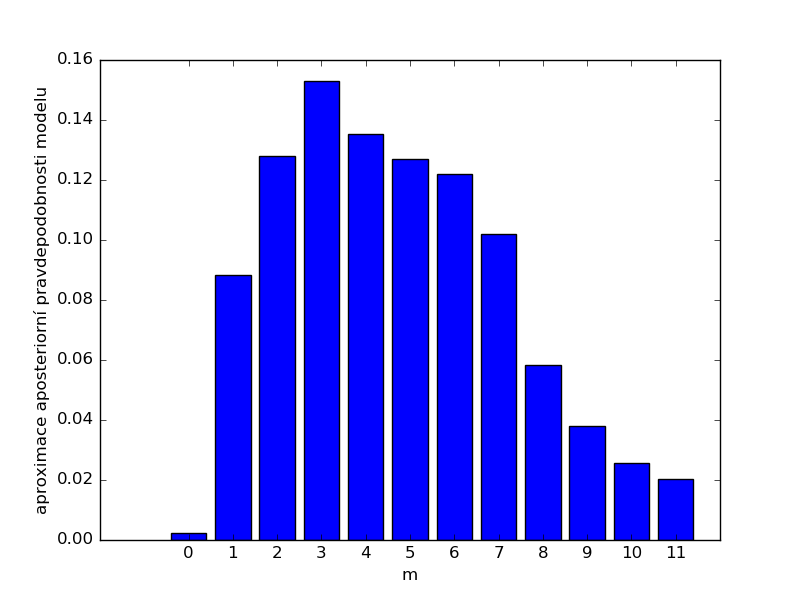
\includegraphics[width=0.8\textwidth]{images/priklad3_20n_hist.png}\caption{Počet dat 20.}\label{model1}
\end{figure}

\begin{figure}
	[H]\centering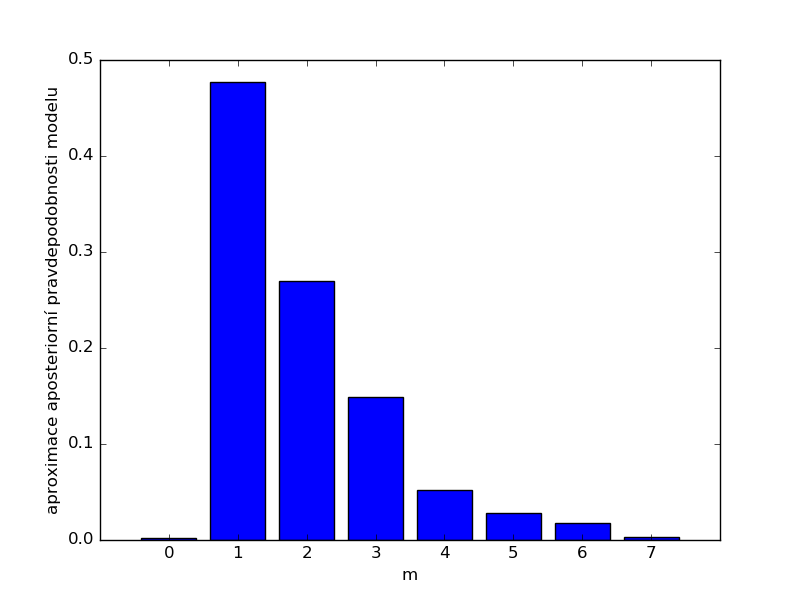
\includegraphics[width=0.8\textwidth]{images/priklad3_50n_hist.png}\caption{Počet dat 50.}
\end{figure}

\begin{figure}
	[H]\centering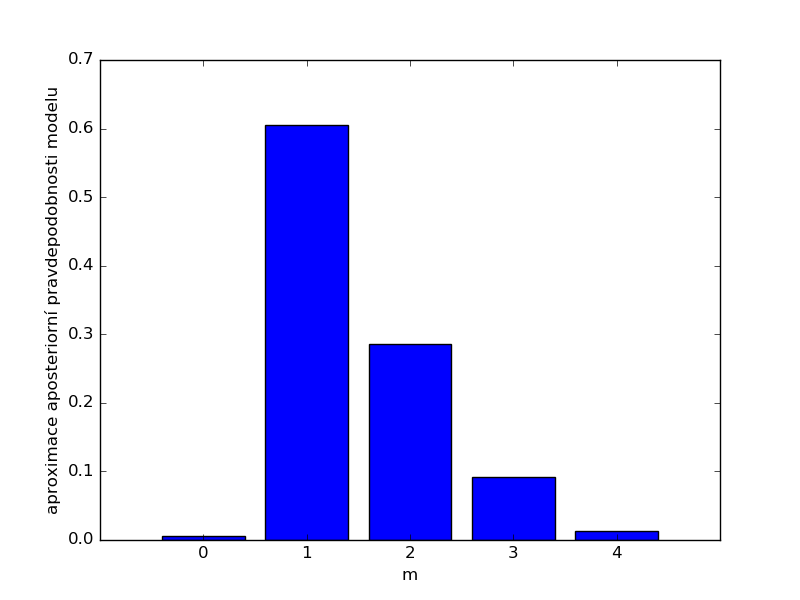
\includegraphics[width=0.8\textwidth]{images/priklad3_100n_hist.png}\caption{Počet dat 100.}\label{model3}
\end{figure}



Z obrázků \ref{model1} až \ref{model3} je vidět, kterým modelům algoritmus dává větší pravděpodobnost s přibývajícím počtem dat. S malým počtem dat algoritmus favorizuje model s větším počtem zlomů, ale čím víc dat máme tím víc se pravděpodobnost modelu přesouvá k modelu s jedním zlomem. Algoritmu stačí 100 vzorků, aby si byl na 60\% jistý modelem 1.

\begin{figure}
	[H]\centering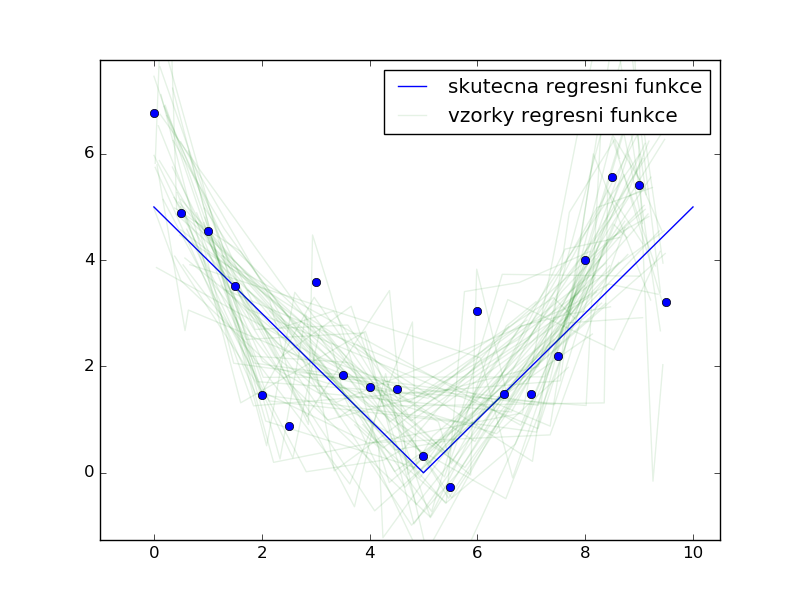
\includegraphics[width=0.8\textwidth]{images/priklad3_20n_lines.png}\caption{Vzorky pro 20 pozorování.}\label{priklad3_lines_20}
\end{figure}

\begin{figure}
	[H]\centering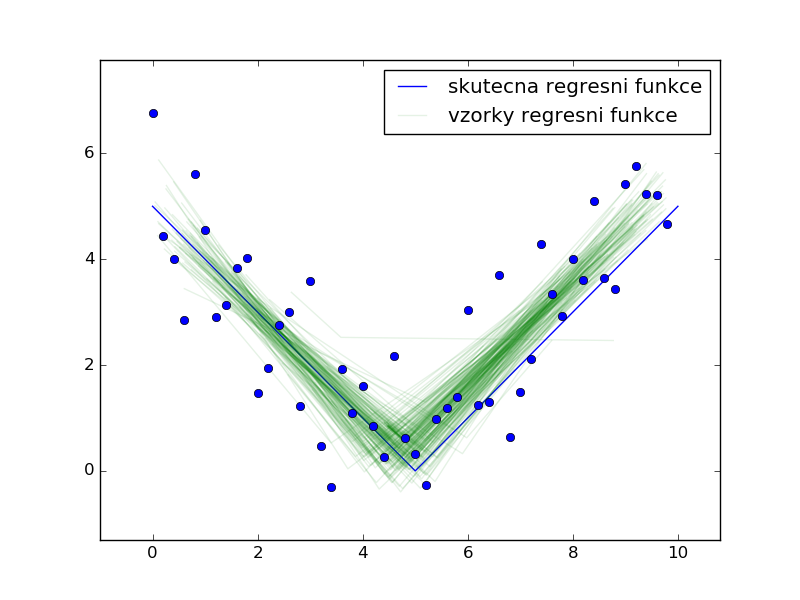
\includegraphics[width=0.8\textwidth]{images/priklad3_50n_lines.png}\caption{Vzorky pro 50 pozorování.}\label{priklad3_lines_50}
\end{figure}

\begin{figure}
	[H]\centering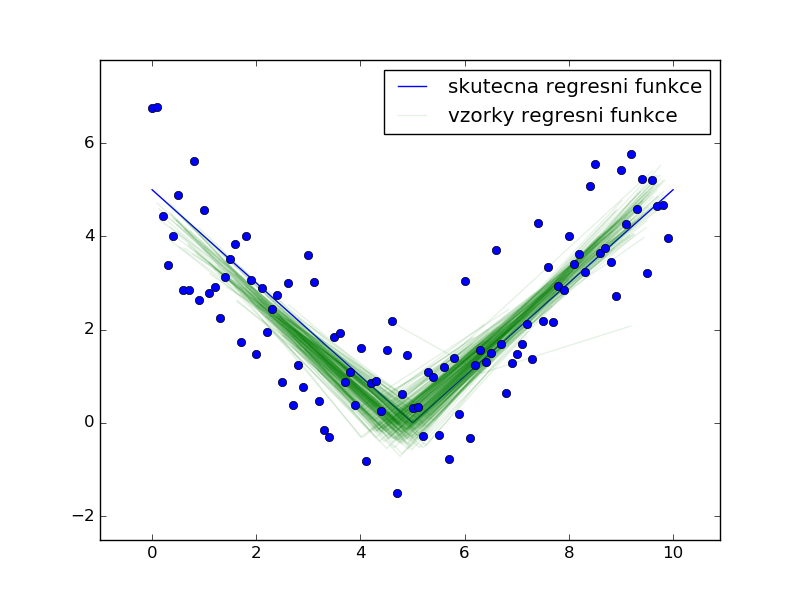
\includegraphics[width=0.8\textwidth]{images/priklad3_100n_lines.png}\caption{Vzorky pro 100 pozorování.}\label{priklad3_lines_100}
\end{figure}

Obrázky \ref{priklad3_lines_20}, \ref{priklad3_lines_50}, \ref{priklad3_lines_100} znázorňují aproximaci aposteriorní distribuce pro nejpravděpodobnější model pro úlohy s 20, 50, 100 daty. Modré tečky představují data s náhodným šumem vygenerované z funkce znázorněné modrou čarou.  \par
V úloze s 20 daty (obrázek \ref{priklad3_lines_20} )je  vidět, že vzorky z dané aposteriorní distribuce se snaží projít co nejvíce body, tudíž špatně aproximují skutečnou regresní funkci. Je to dané malým počtem dat a tím pádem modely s více zlomy vysvětlují data o hodně lépe, než by mohly modely s malým počtem zlomů. Toto se mění na dalších příkladech. Na úloze se 100 daty (obrázek \ref{priklad3_lines_50}) je jasně patrné, že vzorky už jsou rozděleny velmi blízko funkci z které se data generují. Distribuce jsou koncentrovány prakticky skoro přesně na skutečné funkci.

\subsection{Příklad 2}
V druhém příkladu budeme data generovat z funkce dané body $(0, 5), (5, 0), (10, 0), (15, 5)$. Data budou generována s rozptylem 3. Tentokrát jsme z funkce vygenerovali vždy 50 dat a aposteriorní distribuci jsme opět aproximovali 20000 vzorky. Tentokrát jsme změnili apriorní distribuci na rozptylu, kde v jednom případě je $\sigma^2 \sim \mathcal{N}(0, 3)$, v druhém $\sigma^2 \sim \mathcal{N}(3, 0.2)$, ve třetím $\sigma^2 \sim \mathcal{U}(0, 10)$.  První vzorek je $(1, 0, 3, 9.5, 3)$. \par

\begin{figure}
	[H]\centering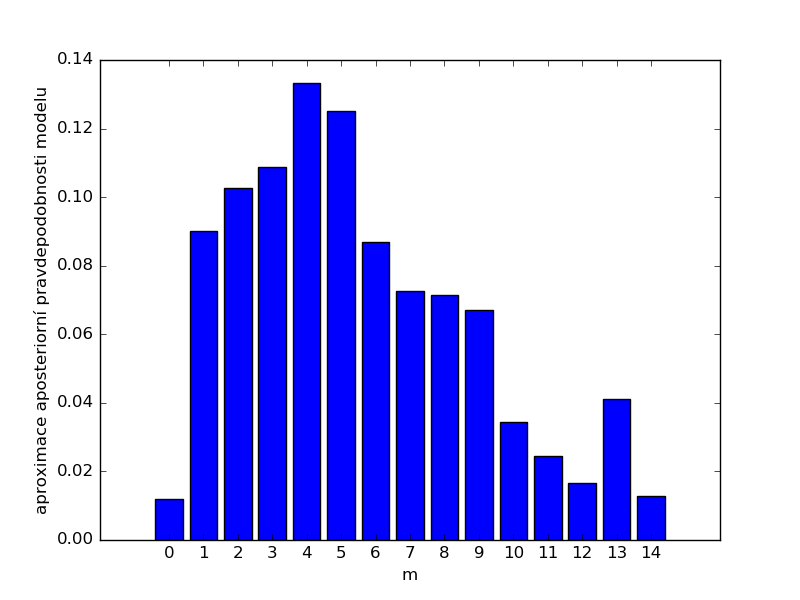
\includegraphics[width=0.8\textwidth]{images/priklad4_N03_hist.png}\caption{$\sigma^2 \sim \mathcal{N}(0, 3)$}\label{sigmaN03}
\end{figure}

\begin{figure}
	[H]\centering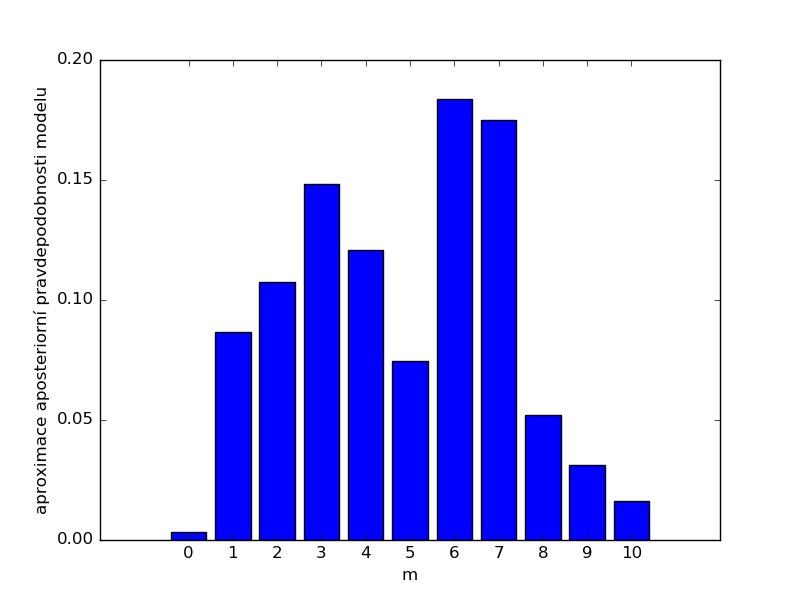
\includegraphics[width=0.8\textwidth]{images/priklad4_N302_hist.png}\caption{$\sigma^2 \sim \mathcal{N}(3, 0.2)$}\label{sigmaN30}
\end{figure}

\begin{figure}
	[H]\centering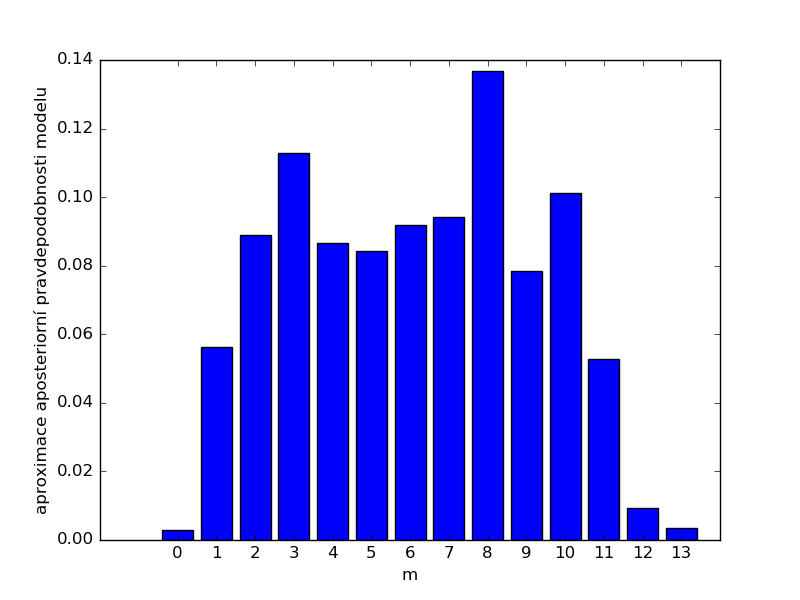
\includegraphics[width=0.8\textwidth]{images/priklad4_U010_hist.png}\caption{$\sigma^2 \sim \mathcal{U}(0, 10)$}\label{sigmaU010}
\end{figure}

\begin{figure}
	[H]\centering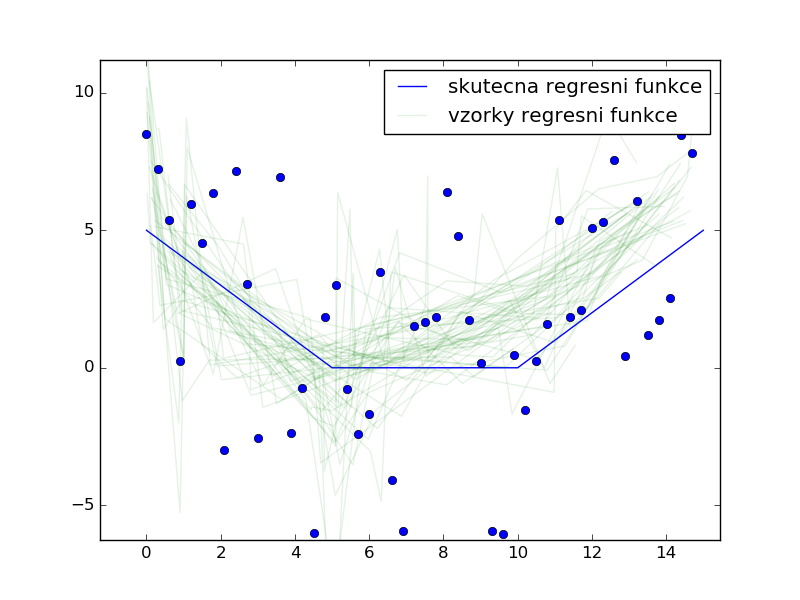
\includegraphics[width=0.8\textwidth]{images/priklad4_N03_lines.png}\caption{Vzorky  modelu se 4 zlomy pro $\sigma^2 \sim \mathcal{N}(0, 3)$}\label{sigmaU010}
\end{figure}

\begin{figure}
	[H]\centering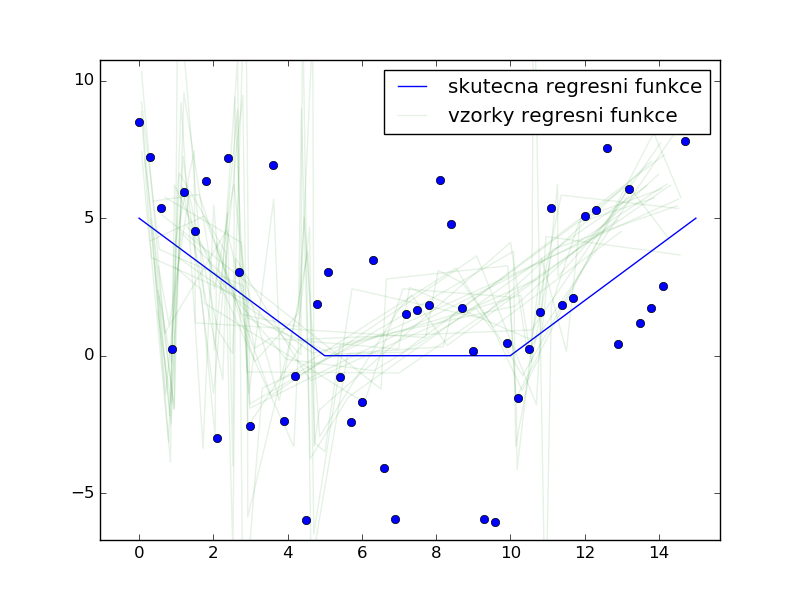
\includegraphics[width=0.8\textwidth]{images/priklad4_N302_lines2.png}\caption{Vzorky  modelu s 6 zlomy pro $\sigma^2 \sim \mathcal{N}(3, 0.2)$}\label{sigmaU010}
\end{figure}

\begin{figure}
	[H]\centering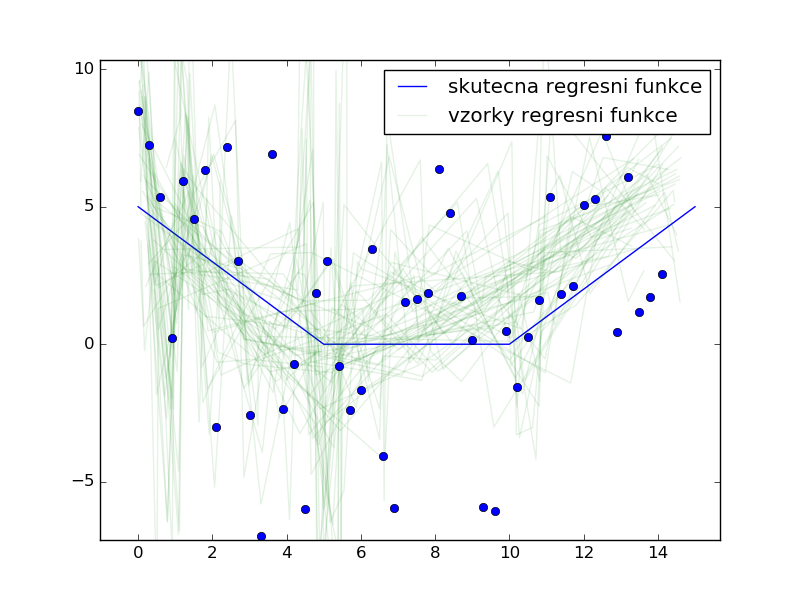
\includegraphics[width=0.8\textwidth]{images/priklad4_U010_lines8.png}\caption{Vzorky modelu s 8 zlomy pro $\sigma^2 \sim \mathcal{U}(0, 10)$}\label{sigmaU010}
\end{figure}

Na obrázcích \ref{sigmaN03} až \ref{sigmaU010} je vidět jak jednotlivé apriorní rozdělení ovlivňují aposteriorní pravděpodobnost modelu. Překvapivé je, že i přesto, že apriorní rozdělení je blízko nuly, tak algoritmus preferuje modely s relativně malým počtem zlomů. Toto bude dáno poměrně velkým rozptylem. U rozdělení $\sigma^2 \sim \mathcal{N}(3, 0.2)$ bychom čekali, že se bude držet spíš u modelů s malým počtem zlomů. Samotné vzorky jsou velmi daleko od skutečného regresního modelu, což je dáno malým počtem vzorků a velkým rozptylem dat.
%\subsection{obsolete}
% \par \par
%  Simulované data pro tento příklad jsou $x = (0, 1, 2, 3, 4, 5, 6, 7, 8, 9, 10)$, $y = (12 + e_1, 10 + e_2, 8 + e_3, 6 + e_4, 4 + e_5, 2 + e_6, 4 + e_7, 6 + e_8, 8 + e_9, 10 + e_10, 12 + e_11)$, kde $e_i \sim \mathcal{N}(0, 0.1)$. Algoritmus jsme nechali běžet o 20000 iterací. A prvotní vzorek je náhodně vygenerovaný vzorek začínající v modelu beze zlomu. 
%\begin{figure}
%	[H]\centering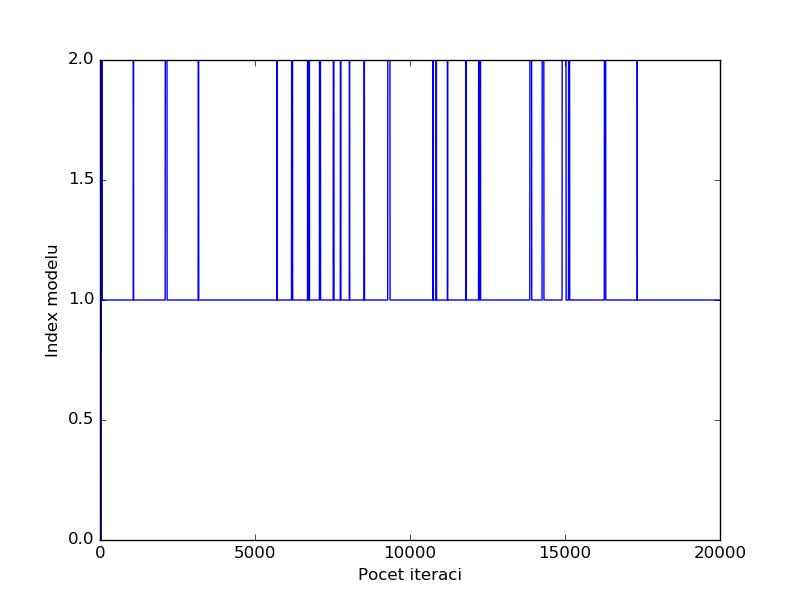
\includegraphics[width=0.8\textwidth]{images/ks_example_V.png}\caption{Vykreslení přeskoku mezi dimenzemi}\label{priklad1_prechody}
%\end{figure} \par
%Z vykreslení přeskoků mezi dimenzemi \ref{priklad1_prechody} je patrné, že algoritmus zůstává v modelu beze zlomu (index 0), prakticky jen nezbytně dlouho dobu než dostane možnost přeskočit do jiné dimenze a poté se už do modelu beze zlomu nikdy nevrací. Poté sice přeskakuje mezi modelem s jedním a dvěma zlomy, ale většinu času stráví v modelu s jedním zlomem. Celkově algoritmus získal 39 vzorků v modelu beze zlomu, 19233 v modelu s jedním zlomem a 728 vzorků v modelu s dvěma zlomy.
%\begin{figure}
%	[h]\centering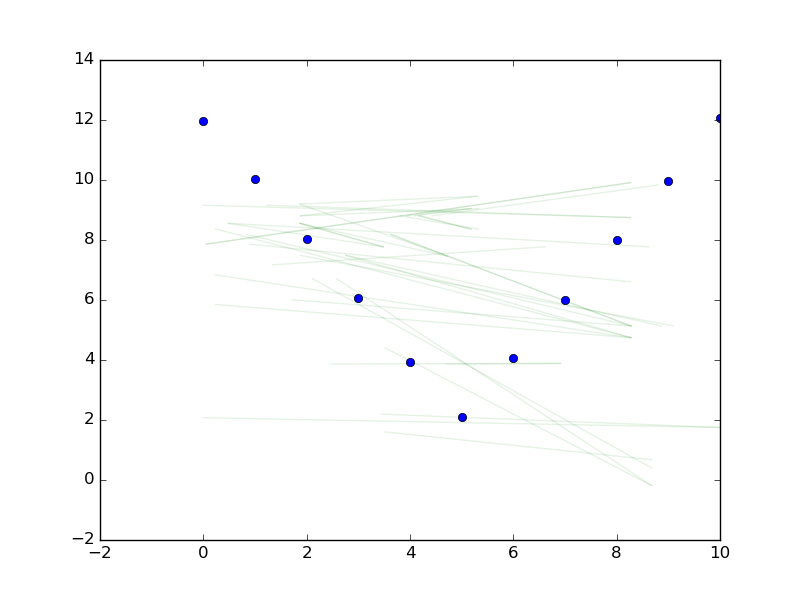
\includegraphics[width=0.8\textwidth]{images/distribution_lines_v_0breaks.png}\caption{%Aproximace distribuce modelu beze zlomu}\label{v0break}
%\end{figure}
%\begin{figure}
%	[H]\centering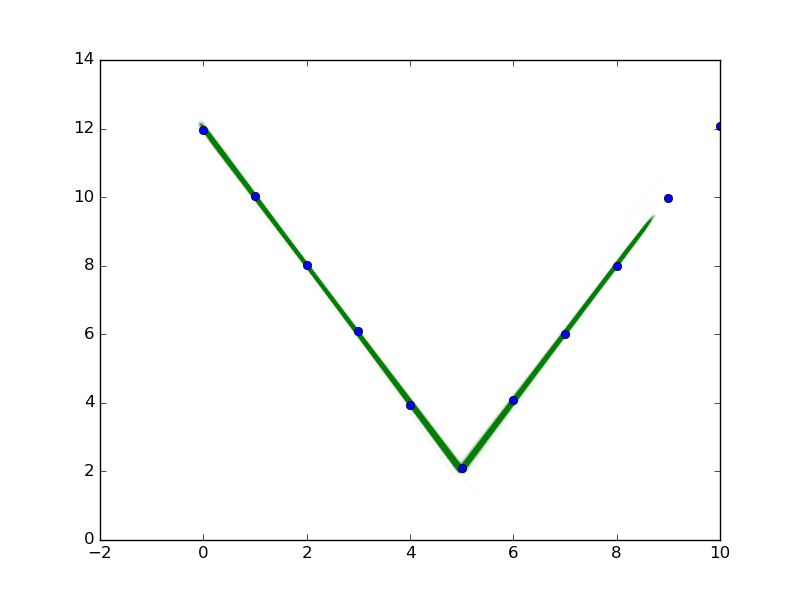
\includegraphics[width=0.8\textwidth]{images/distribution_lines_V_1break.png}\caption{Aproximace distribuce modelu s jedním zlomem}\label{v1break}
%\end{figure}
%\begin{figure}
%	[H]\centering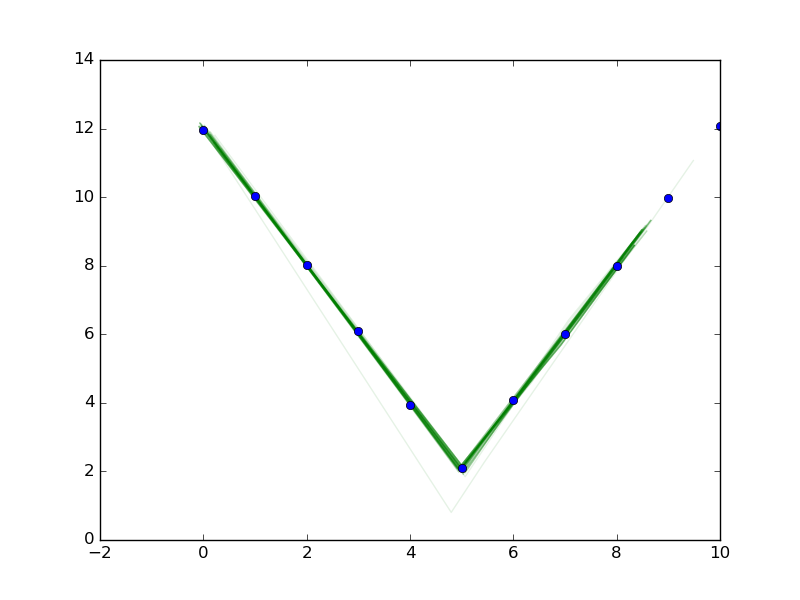
\includegraphics[width=0.8\textwidth]{images/distribution_lines_V_2breaks.png}\caption{Aproximace distribuce modelu s dvěma zlomy}\label{v2break}
%\end{figure} \par
%Na obrázcích \ref{v0break}, \ref{v1break}, \ref{v2break} můžeme vidět aproximace distribucí pro dané modely, pomocí vzorků z jednotlivých modelů. Zajímavé je si všimnou, faktu, že i když distribuce pro model s jedním respektive dvěma zlomy vypadají podobně, tak algoritmus strávil mnohem víc času v modelu s jedním zlomem. Je to právě dáno bayesovským přístupem, který zvýhodňuje jednodušší modely se stejnou vysvětlovací schopností. \par
%Ukážeme si ještě jeden příklad a to se stejnými $x = (0, 1, 2, 3, 4, 5, 6, 7, 8, 9, 10)$ jako minule, ale $y = (20 + e_1, 15 + e_2, 7 + e_3, 1 + e_4, 1 + e_5, 1 + e_6, 1 + e_7, 11 e_8, 18 + e_9 ,25 + e_10, 32 + e_11)$ a $e_i \sim \mathcal{N}(0, 0.1)$ respektive $e_i \sim \mathcal{N}(0, 2)$. \par
%V prvním případě algoritmus prakticky okamžitě přechází do modelu s dvěma zlomy a už z něj nevychází, počet vzorků v modelu 0 je 65, modelu 1 78, modelu 2 19857. V případě s vyšší dimenzí je rozdíl a to, že o hodně častěji algoritmus přechází do modelu 1. Počet vzorků v modelu 0 je 38, modelu 1 4039, modelu 2 15923. Na obrázku \ref{priklad2_prechody} je vidět jak algoritmus přechazí mezi jednotlivými modely.
%\begin{figure}
%	[H]\centering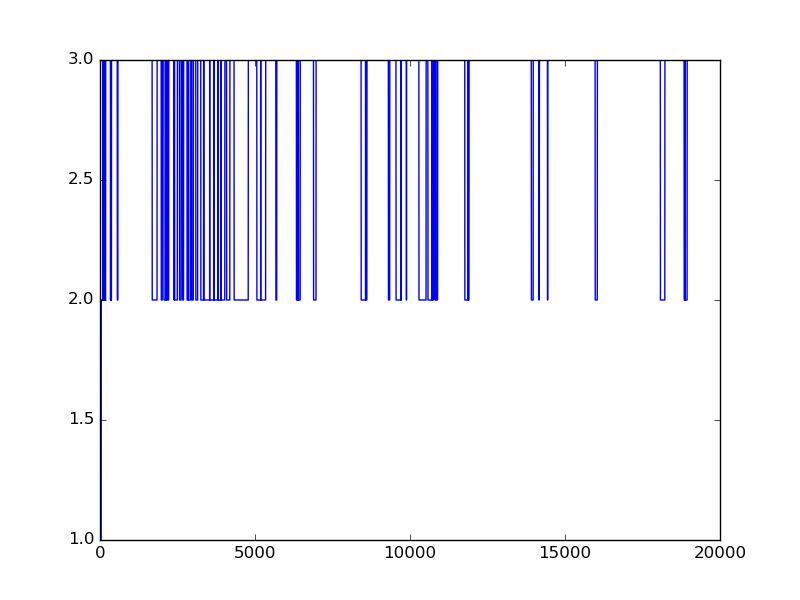
\includegraphics[width=0.8\textwidth]{images/ks_examle_u_bigger_variance.png}\caption{Vykreslení přeskoku mezi dimenzemi příklad 2, $\sigma^2 = 2$}\label{priklad2_prechody}
%\end{figure}
%\begin{figure}
%	[H]\centering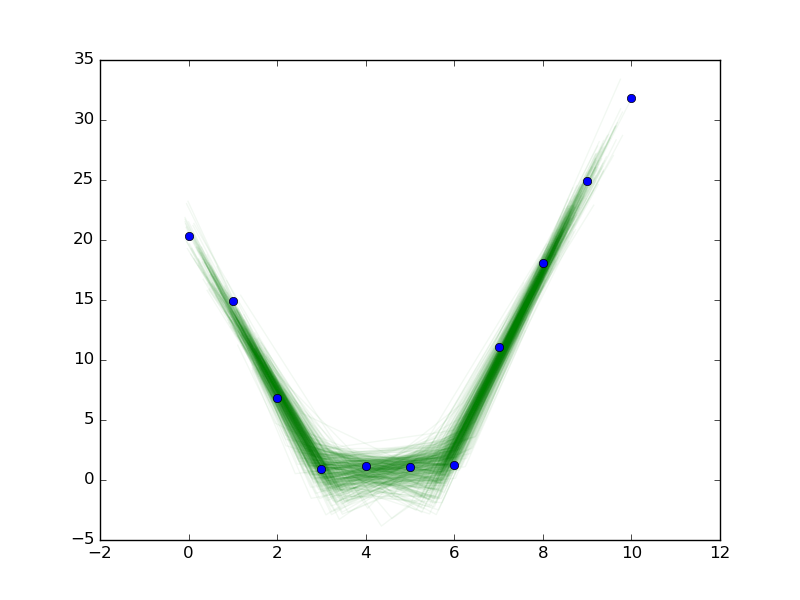
\includegraphics[width=0.8\textwidth]{images/distribution_lines_u_2breaks_small_variance.png}\caption{Aproximace distribuce modelu s dvěma zlomy, $\sigma^2 = 0.1$}\label{priklad2_distribuce_small_sigma}
%\end{figure}
%\begin{figure}
%	[H]\centering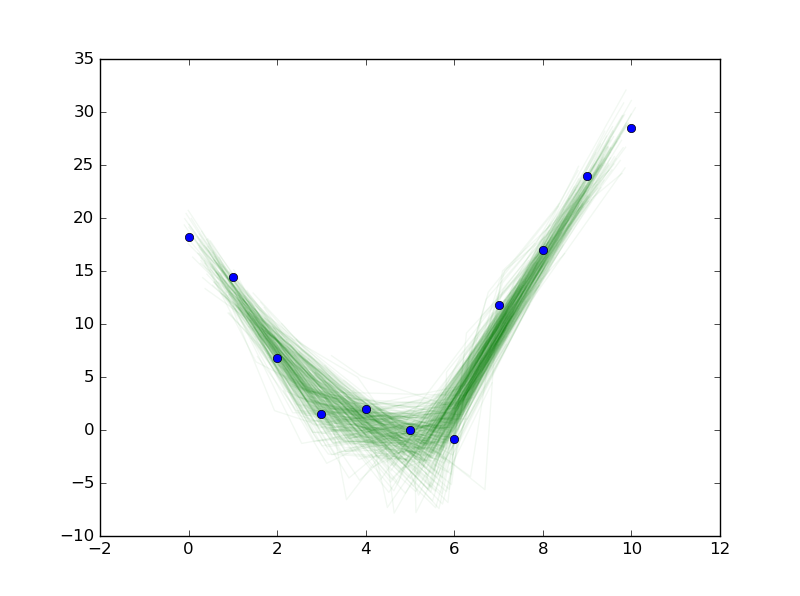
\includegraphics[width=0.8\textwidth]{images/distribution_lines_u_2breaks_bigger_variance.png}\caption{Aproximace distribuce modelu s dvěma zlomy, $\sigma^2 = 2$}\label{priklad2_distribuce_big_sigma}
%\end{figure}
%Na obrázcích \ref{priklad2_distribuce_small_sigma}, \ref{priklad2_distribuce_big_sigma} je vidět distribuce s menším respektive větším rozptylem. Na distribuci s menším rozptylem je vidět, že mnohem více koncentrována kolem skutečných bodů zlomu, což jsou body 3 a 6. A naopak distribuce s větším rozptylem není tak moc koncentrovaná, jak se dalo čekat.



\section{Zdrojové kódy}
Velkou částí této práce byla samotná implementace algoritmu RJMCMC a proto si zde ukážeme nejdůležitější části samotné implementace. Jedním z největších problémů bylo jak pro každý model vygenerovat samotné aposteriorní distribuce, přechody do modelů s větším nebo menším počtem zlomů a vzorkovače pro přechody v rámci daného modelu. Dalším problémem je, jak pro přechodové funkce $h_p$ generovat odpovídající jakobiány, ručně by to bylo možné, ale obzvlášť ve vyšších dimenzích náročné na manuální chyby a i samotná implementace by se ztížila. Proto jsme pro implementaci přechodových funkcí zvolili knihovnu Theano\cite{theano}, která dokáže symbolicky spočítat jakobiány a tím nám ušetří práci navíc. \par

\begin{lstlisting}[label=blr, caption=Blr]
class Blr:
    '''
    Trida, ktera vytvori stacionarni distribuci pro regresi s n zlomy.
    2 protoze pouzivam jinou parametrizaci.
    sigma = x[0] - rozptyl 
    s0 = x[1] - xova souradnice prvniho zlomu
    h0 = x[2] - yova souradnice prvnhio zlomu
    ...
    sn = x[n-2] - xova souradnice nteho zlomu
    hn = x[n-1] - yova souradnice nhteo zlomu
    '''

    def __init__(self, xs, ys, n_breaks):
        '''
        @param xs - xove souradnice dat
        @param ys - yove souradnice dat
        @param n_breaks - pocet zlomu
        '''
        if not (len(xs) == len(ys)):
            raise RuntimeError("Not matching dimension. Dimension xs=" + str(len(xs)) + " Dimension ys=" + str(len(ys)))
        self.xs = xs
        self.ys = ys
        self.max_x = max(xs)
        self.min_x = min(xs)
        self.n = 2*n_breaks + 5
        self.n_samples = len(xs)
        self.max_y = max(ys)
        self.min_y = min(ys)
        self.h_prior = uniform(self.min_y - 1, self.max_y + 1)
        self.sigma_prior = normal(0, 3)
        self.n_breaks = n_breaks
        
    def prior_s(self, theta):
        '''
        Apriorni rozdeleni na thetaovych souradnicich. Tedy melo by platit
        ss < s1 < s2 < ... < sn < sf. Je to tak nastaveno z toho duvodu,
        aby bylo dodrzeni poradi
        '''
        x_coordinates = [theta[i] for i in range(1, self.n, 2)]
        previous = x_coordinates[0]
        for i in range(1, len(x_coordinates)):
            if previous > x_coordinates[i]:
                return 0
            previous = x_coordinates[i]

        if x_coordinates[0] < self.min_x - 0.1:
            return 0
        if x_coordinates[len(x_coordinates) - 1] > self.max_x + 0.1:
            return 0
        return 1

    def prior_h(self, theta):
        '''
        Apriorni rozdeleni na yovych souradnicich. Je teda co nejvic
        neinformativni, tedy pro vsechny h plati, ze h ~ U(y_min - 1, y_max + 1)
        '''
        y_coordinates = [theta[i] for i in range(2, self.n, 2)]
        return np.prod(self.h_prior.pdf(y_coordinates))

    def prior_sigma(self, theta):
        '''
        Apriorni rozdeleni na rozptylu. Zas jen nake neinformativni a s
        nulovou pravdepodobnosti na sigmach mensi nez 0
        '''
        if theta[0] > 0:
            return self.sigma_prior.pdf(theta[0])
        return 0

    def likelihood(self, theta):
        '''
        Spocita likelihood hustotu pro dany vzorek
        '''
        assert len(theta) == self.n

        suma = 0
        for i, xi in enumerate(self.xs):
            yi = self.ys[i]
            for j in range(1, self.n-2, 2):
                break1 = (theta[j], theta[j+1])
                break2 = (theta[j+2], theta[j+3])

                if break1[0] <= xi < break2[0]:
                    suma += self.prob_sum(xi, yi, break1, break2)

            # tohle je pro pripad ze xi je pred nebo za body urcujicimi primku
            # stava se to :D
            if xi < theta[1]:
                break1 = (theta[1], theta[2])
                break2 = (theta[3], theta[4])
                suma += self.prob_sum(xi, yi, break1, break2)

            if xi > theta[self.n - 2]:
                break1 = (theta[self.n-4], theta[self.n-3])
                break2 = (theta[self.n-2], theta[self.n-1])
                suma += self.prob_sum(xi, yi, break1, break2)

        try:
            exp = np.exp(-suma/(2*theta[0]))
            bs = theta[0]**(-len(self.xs)/2)
            return bs * exp
        except FloatingPointError:
            print()
            print('theta0 ' + str(theta[0]))
            print('suma ' + str(suma))
            return 0

    def prob_sum(self, x, y, break1, break2):
        '''
        pomocna funkce, co mi spocita jeden vyraz v exponenciale, jakoze v
        Normalnim rozdeleni hore
        '''

        # a = (break2[1] - break1[1])/(break2[0]-break1[0])
        # b = break2[1] - break2[0]*a
        x1, y1 = break1
        x2, y2 = break2
        est = (x - x1)*(y2 - y1)/(x2 - x1) + y1
        return (y - est)**2

    def pdf(self, theta):
        if len(theta) is not self.n:
            print(theta)
            raise Exception("Co  to")

        prior_probs = np.prod([self.prior_h(theta),
                               self.prior_s(theta),
                               self.prior_sigma(theta)])

        # netkere vzorky budou mit nulovou pravdepodobnost
        # uz kvuli apriornimu rozdeleni, proto to checknu
        # at se nemusi pocitat likelihood ten v zavislosti
        # na datech muze byt dost narocny spocitat
        if prior_probs == 0:
            return 0
        return np.prod([prior_probs,
                        self.likelihood(theta)])

    def generate_first_sample(self):
        '''
        vygeneruje nejaky vzorek, ktery nema pravdepodobnost nula
        '''
        minimum = min(self.xs)
        maximum = max(self.xs)
        first_sample = np.zeros(self.n)

        first_sample[0] = 1

        for i, x in enumerate(np.linspace(minimum, maximum, (self.n-1)/2)):
            first_sample[2*i + 1] = x
            first_sample[2*i + 2] = np.random.normal(0, 3)

        if not self.pdf(first_sample) > 0:
            print("First sample: " + str(first_sample) +
                  " has zero probability")
            print("prior h " + str(self.prior_h(first_sample)))
            print("prior s " + str(self.prior_s(first_sample)))
            print("prior sigma " + str(self.prior_sigma(first_sample)))
            print("likelihood " + str(self.likelihood(first_sample)))
            return self.generate_first_sample()

        return first_sample
\end{lstlisting}

Třída Blr \ref{blr} slouží k výpočtům hodnot aposteriorního rozdělení pro daný vzorek. Je napsaná tak, aby fungovala pro jakýkoli počet, ale pevný, počet zlomů. Z toho důvodu je potřeba ji vytvořit zvlášť pro každý model, který se používá v simulaci. 

\begin{lstlisting}[caption=RJMCM]
class Rjmcmc:
    '''
    trida ktera zastitute cely reversible jump markov chain
    monte carlo algoritmus
    '''

    def __init__(self, move_factory, mcmc_factory, stationary_factory):
        self.move_factory = move_factory
        self.mcmc_factory = mcmc_factory
        self.stationary_factory = stationary_factory
        self.trans_steps = 0
        self.norm_steps = 0

    def step(self, previous_sample):
        k, theta = previous_sample
        u = uniform()
        moves = [m for m in self.move_factory.get_moves_from(k) if m.can_move(k) > 0]
        trans_probability = 0
        for m in moves:
            trans_probability += m.probability_of_this_move(previous_sample)
        if u < trans_probability: 
        	# v této části se uskutečňuje pokus o mezi dimenzionální skok
            self.trans_steps += 1
            uu = uniform(0, trans_probability)
            M = None
            prob = 0
            for m in moves:
                if prob < uu < prob + m.probability_of_this_move(previous_sample):
                    M = m
                    break
                prob += m.probability_of_this_move(previous_sample)

            up, down, a, new = self.trans_step(M, previous_sample)
            return new
        else:
        	# v této části se nechá generovat vzorek sampler daného modelu
            self.norm_steps += 1
            if (k+1)*2 + 3 is not len(theta):
                print(k)
                print(previous_sample)
                raise Exception("wrong length")
            return (k, self.mcmc_factory.get_mcmc(k).step(theta))

    def trans_step(self, move, previous_sample):
        (k, theta) = previous_sample

        new_sample, u, newu, det_jacobian = move.transform(previous_sample)

        (new_k, new_theta) = new_sample
        up = np.prod([
            self.stationary_factory.get_stationary(new_k).pdf(new_theta),
            move.probability_of_this_move(new_sample),
            move.probability_of_help_rvs(new_sample, newu)])
        down = np.prod([
            self.stationary_factory.get_stationary(k).pdf(theta),
            move.probability_of_this_move(previous_sample),
            move.probability_of_help_rvs(previous_sample, u)])

        a = det_jacobian*up/down
        u = uniform()

        if u < a:
            return (up, down, a, new_sample)
        else:
            return (up, down, a, previous_sample)

    def sample(self, n, first_sample):
        samples = [first_sample]
        for i in range(1, n):
            new_sample = self.step(samples[i-1])
            samples.append(new_sample)
            # progress bar
            sys.stdout.write("\r\t%.0f%% Done" % (100*i/n))
            sys.stdout.flush()
        # progress konec
        sys.stdout.write("\r\t100% Done\n")
        sys.stdout.flush()
        return samples
\end{lstlisting}

K samotnému běhu algoritmu slouží stejně pojmenována třída. Jako argumenty jejího konstruktoru slouží tři továrny. Jedna je pro výrobu samplerů pro jednotlivé modely, další pro výrobu stacionárních distribuci jednotlivých modelů a poslední pro výrobu samotných přeskoků. Výhodou takovéhoto postupu je, že pokud bychom chtěli aplikovat RJMCM na jiný problém než regresi, stačí si vytvořit továrny pro daný problém a zbytek algoritmu zůstává stejný. 

\begin{lstlisting}[caption=BlrMoveFactory]
class BlrMoveFactory(AbstractMoveFactory):
    def __init__(self):
        self.dimension_to_moves = {}

    def get_moves_from(self, k):
        if k in self.dimension_to_moves.keys():
            return self.dimension_to_moves[k]

        print("Creating moves from " + str(k))
        moves = []
        u = uniform(0, 1)
        n = normal(0, 1)
        # moves up
        for i in range(k+1):
            t_up, j_up = self._create_transformation_up(k, i)
            t_down, j_down = self._create_transformation_down(k+1, i)
            u_gen_up = ProposalDistribution(lambda x: u.pdf(x[0])*n.pdf(x[1]),
                                            lambda: [u.rvs(), n.rvs()])
            move = Move(k, k+1, 0.05/(k+1), 0.05/(k+1),
                        t_up, t_down, j_up, j_down,
                        u_gen_up, None, 2, 0)
            moves.append(move)
        # moves down
        for i in range(k):
            t_up, j_up = self._create_transformation_up(k-1, i)
            t_down, j_down = self._create_transformation_down(k, i)
            u_gen_up = ProposalDistribution(lambda x: u.pdf(x[0])*n.pdf(x[1]),
                                            lambda: [u.rvs(), n.rvs()])
            move = Move(k-1, k, 0.05/k, 0.05/k,
                        t_up, t_down, j_up, j_down,
                        u_gen_up, None, 2, 0)
            moves.append(move)

        self.dimension_to_moves[k] = moves
        return moves

    def _create_transformation_up(self, k, m):
        '''
        k - pocet zlomu
        m - ktery zlom zlomit :D,
            e.g 0 - novy zlom mezi 0. a 1.
                1 - novy zlom mezi 1. a 2.
        '''
        if m < 0 or m > k:
            raise Exception("Nemozno zlomit takto")

        x = T.vector('x')
        # k*2 - kazdy zlom ma dva body, 1 - sigma, 4 - koncove body,
        # 2 - nahodne veliciny
        n = k*2 + 1 + 4 + 2
        f_list = [None for _ in range(n)]
        f_list[0] = x[0]
        break1 = 1 + 2*m + 2
        for i in range(1, break1):
            f_list[i] = x[i]

        f_list[break1] = x[break1-2] + (x[break1]-x[break1-2])*x[n-2]
        f_list[break1+1] = x[break1-1] + (x[break1+1]-x[break1-1])*x[n-2] + x[n-1]

        for i in range(break1+2, n):
            f_list[i] = x[i-2]

        f = T.as_tensor_variable(f_list)
        jacobian = theano.function([x], theano.gradient.jacobian(f, x))

        assert any([y is not None for y in f_list])
        return theano.function([x], f), jacobian

    def _create_transformation_down(self, k, m):
        '''
        k - pocet zlomu
        m - ktery zlom vymazat :D,
            e.g 0 - vymazat zlom mezi 0. a 2.
                1 - vymazat zlom mezi 1. a 3.
        '''
        if m < 0 or m >= k:
            raise Exception("Nemozno vymazat takto")

        x = T.vector('x')
        # k*2 - kazdy zlom ma dva body, 1 - sigma, 4 - koncove body,
        n = k*2 + 1 + 4
        f_list = [None for _ in range(n)]
        f_list[0] = x[0]
        break1 = 1 + 2*m + 2

        for i in range(1, break1):
            f_list[i] = x[i]

        for i in range(break1, n-2):
            f_list[i] = x[i+2]

        f_list[n-2] = (x[break1] - x[break1-2])/(x[break1+2] - x[break1-2])
        f_list[n-1] = x[break1+1] - x[break1-1] - (x[break1+3] - x[break1-1])*(x[break1] - x[break1-2])/(x[break1+2] - x[break1-2])

        f = T.as_tensor_variable(f_list)
        jacobian = theano.function([x], theano.gradient.jacobian(f, x))

        assert any([y is not None for y in f_list])
        return theano.function([x], f), jacobian
\end{lstlisting}

BlrMoveFactory slouží k vytváření přechodů mezi modely. K implementaci transformačních funkcí používáme knihovnu Theano\cite{theano}, její výhodou je, že dokáže symbolicky počítat jakobiány. Pro to je ale potřeba nejdříve vygenerované funkce zkompilovat a tento proces může zabrat nějaký čas. Z toho důvodu se vyplatí si vytvořené přechody ukládat do hash mapy a když jsou znovu potřeba, tak jen znovu vrátit už vytvořené přechody. Další výhodou této třídy je, že přechody se vygenerují vždy jen, když jsou potřeba.

\begin{lstlisting}[caption=McmcFactory]
class McmcFactory:
    def __init__(self, stationaryDistributionFactory):
        self.dimension2mcmc = {}
        self.stat_factory = stationaryDistributionFactory

    def get_mcmc(self, k):
        if k in self.dimension2mcmc.keys():
            return self.dimension2mcmc[k]
        blr = self.stat_factory.get_stationary(k)
        prop = ProposalDistribution2(normal(np.zeros(blr.n), 5*np.eye(blr.n)))
        mcmc = Mcmc(prop, blr)
        self.dimension2mcmc[k] = mcmc
        return mcmc
\end{lstlisting}
\begin{lstlisting}[caption=StationaryDistributionFactory]
class StationaryDistributionFactory:
def __init__(self, xs, ys):
self.xs = xs
self.ys = ys
self.dimension2stationary = {}

def get_stationary(self, k):
if k in self.dimension2stationary.keys():
return self.dimension2stationary[k]
blr = Blr(self.xs, self.ys, k)
self.dimension2stationary[k] = blr
return blr
\end{lstlisting}

Třída McmcFactory respektive StationaryDistributionFactory  slouží k vytváření samplerů respektive stacionárních distribuci pro jednotlivé modely. Opět se jednou vytvořené objekty ukládají, tak aby se daly znovu použít. 

\begin{lstlisting}[caption=Move]
class Move:
    '''
    predstavuje prechod z k do k' a zpet
    '''

    def __init__(self,
                 k1,
                 k2,
                 k1_to_k2,
                 k2_to_k1,
                 transform1to2,
                 transform2to1,
                 jacobian1to2,
                 jacobian2to1,
                 ugenerator1to2,
                 ugenerator2to1,
                 usize1,
                 usize2):
        '''
        k1 - prvni stav
        k2 - druhy stav
        k1_to_k2 - pravdepodobnost prechodu z k1 do k2
        k2_to_k1 - pravdepodobnost prechodu z k2 do k1
        transform1to2 - pretransformuje vzorek na vzorek s jinou dimenzi
                        vraci novy vzorek a mozne nahodne cisla, ktere
                        by byly vegenerovane pro zpetnou transformaci
        transform2to1 - ---||---
        ugenerator1to2 - generator pomocnych nahodnych velicin pro prechod
                         z k1 do k2
        ugenerator2to1 - ---||---
        usize1 - delka vektoru nahodnych velicin ktery se vygeneruje pro prechod ze 
                 stavu 1 do stavu 2
        usize2 - ---||---
        '''
        self.k1 = k1
        self.k2 = k2
        self.k1_to_k2 = k1_to_k2
        self.k2_to_k1 = k2_to_k1
        self.transform1to2 = transform1to2
        self.transform2to1 = transform2to1
        self.jacobian1to2 = jacobian1to2
        self.jacobian2to1 = jacobian2to1
        self.ugenerator1to2 = ugenerator1to2
        self.ugenerator2to1 = ugenerator2to1
        self.usize1 = usize1
        self.usize2 = usize2

    def can_move(self, k):
        '''
        urci jestli muzu pouzit tento prechod z daneho stavu
        '''
        if k == self.k1:
            return self.k1_to_k2
        elif k == self.k2:
            return self.k2_to_k1
        else:
            return 0

    def probability_of_this_move(self, x):
        '''
        pravdepodobnost pouziti tohole typu pohybu z daneho
        stavu. zatim pouzivame jen dany stav k, ale v algoritmu
        je mozne i pouzit pro vypocet pravdepodobnosti soucasny
        vzorek. takze ted ty prechodove pravdepodobnosti jsou jenom
        konstanty, ale obecne by to mohla byt i funkce
        '''
        k, theta = x
        if self.k1 == k:
            return self.k1_to_k2
        elif self.k2 == k:
            return self.k2_to_k1
        else:
            raise RuntimeError("This should never happen")

    def _transform(self, k, newk, theta, generator, transform, newu_size):
        if generator is not None:
            u = generator.rvs()
            ext_theta = np.append(theta, u)
        else:
            u = None
            ext_theta = theta
        newtheta = transform(ext_theta)

        if newu_size is not 0:
            newu = newtheta[-newu_size:]
            newtheta = newtheta[:-newu_size]
        else:
            newu = None
        newx = (newk, newtheta)
        det_jacobian = self.get_jacobian((k, ext_theta))
        return (newx, u, newu, det_jacobian)

    def transform(self, x):
        k, theta = x
        if self.k1 == k:
            return self._transform(k,
                                   self.k2,
                                   theta,
                                   self.ugenerator1to2,
                                   self.transform1to2,
                                   self.usize2)
        elif self.k2 == k:
            return self._transform(k,
                                   self.k1,
                                   theta,
                                   self.ugenerator2to1,
                                   self.transform2to1,
                                   self.usize1)
        else:
            raise RuntimeError("This shoould never happen")

    def probability_of_help_rvs(self, x, u):
        k, theta = x
        if self.k1 == k:
            if self.ugenerator1to2 is None:
                return 1
            return self.ugenerator1to2.pdf(u)
        elif self.k2 == k:
            if self.ugenerator2to1 is None:
                return 1
            return self.ugenerator2to1.pdf(u)
        else:
            raise RuntimeError("This should never happen")

    def get_jacobian(self, x):
        k, theta = x
        if self.k1 == k:
            mat = self.jacobian1to2(theta)
            return np.linalg.det(mat)
        elif self.k2 == k:
            mat = self.jacobian2to1(theta)
            return np.linalg.det(mat)
        else:
            raise RuntimeError("This should never happen")
\end{lstlisting}

Move je třída, která shrnuje všechny potřebné funkce k přechodu do jiného modelu a zpátky, tj. transformační funkce, jakobiány transformačních funkcí, generátory náhodných veličin, pravděpodobnosti přechodu. 

\begin{lstlisting}[caption=Vzorkovač]
class Mcmc:
    def __init__(self, proposalDistribution, stationaryDistribution):
        self.proposal = proposalDistribution
        self.stationary = stationaryDistribution

    def step(self, previous_sample):
        '''
        Vnitrek mcmc algoritmu, prakticky to co se deje v jedne 
        iteraci tady te verze hastingse
        '''
        proposal_sample = self.proposal.rvs(previous_sample)
        assert proposal_sample is not None
        local_previous_sample = copy.copy(previous_sample)
        final_sample = copy.copy(previous_sample)

        for j, x in enumerate(proposal_sample):
            local_previous_sample[j] = x
            down = np.prod([
                self.stationary.pdf(previous_sample),
                self.proposal.pdf(local_previous_sample, previous_sample)])
            up = np.prod([
                self.stationary.pdf(local_previous_sample),
                self.proposal.pdf(previous_sample, local_previous_sample)])

            u = np.random.uniform()

            if u < up/down:
                final_sample[j] = x
            else:
                local_previous_sample[j] = previous_sample[j]

        return final_sample

    def sample(self, n, first_sample):
        dimension = len(first_sample)
        samples = np.empty((n, dimension))
        samples[0] = first_sample
        for i in range(1, n):
            samples[i] = self.step(samples[i-1])
            # progress bar
            sys.stdout.write("\r\t%.0f%% Done" % (100*i/n))
            sys.stdout.flush()
        # progress konec
        sys.stdout.write("\r\t100% Done\n")
        sys.stdout.flush()
        return samples
\end{lstlisting}

Mcmc je třída pro vzorkování. Použitý algoritmus je jedna varianta Metropolisova-Hastingsova algoritmu, která vzorky přijímá postupně po jednotlivých částech parametru, čímž dosahuje větší pravděpodobností přijetí. 
\section{Závěr}
V práci jsme stručně popsali problémy, které se pojí s odhadováním parametrů modelů s proměnnou dimenzí. Začali jsme úvodem do Bayesovské statistiky, poté jsme zavedli model pro po částech lineární regresi. Následně jsme si ukázali jak fungují MCMC algoritmy, které ale samy o sobě nejsou dostačující pro dosažení závěrů o našem modelu, proto jsme přešli k algoritmu RJMCMC. Ten dokáže aproximovat aposteriorní rozdělení u modelů, kde jeden z parametrů je počet ostatních parametrů. Stručně jsme popsali to, jak algoritmus RJMCMC řeší problém s přechodem mezi dimenzemi a ukázali jsme, jak by takové přechody mohly vypadat. \par
Značná část naší práce spočívá v samotné implementaci algoritmu RJMCMC. Ten jsme naprogramovali v jazyce Python za pomocí knihoven NumPy a SciPy, které se používají obecně k vědeckým výpočtům a v našem případě konkrétně jsme je použili pro simulaci dat z různých pravděpodobnostních rozdělení. Také jsme použili knihovnu Theano, která slouží k symbolickým výpočtům derivací a v našem případě Jakobiánu. Na závěr naší práce jsme předvedli funkčnost naší implementace algoritmu na simulovaných datech a na výsledcích ilustrovali a popsali typické rysy bayesovského přístupu k volbé modelu. \par
Naše implementace algoritmu RJMCMC je dosti obecná, přirozeným pokračováním naší práce by bylo vyzkoušení daného algoritmu na jiných problémech, jako například rozpoznávaní obrazů nebo pro směsi normálních rozdělení. Dále by si tato práce zasloužila rozvést teoretickou stránku fungování algoritmu. Protože většina reálných problému nezávisí jen na jedné veličině, bylo by dalším zajímavým rozšířením pokusit se implementovat algoritmus RJMCMC pro více dimenzionální lineární regresi. Toto by už by mohlo být značně náročné z hlediska návrhu návrhových distribucí. 

\bibliographystyle{plain}
\bibliography{bibliography}


\end{document}

 
